\setchapterpreamble[u]{\margintoc}
\chapter{Findings: Mobile Analytics Tools and their Artefacts}~\label{chapter-tools-and-their-artefacts}
This chapter covers two of the six perspectives, \emph{i.e.} using and improving mobile analytics tools. The primary evidence comes from both the app-centric and the tool-centric case studies, augmented with material from grey data and grey literature.

The evidence has been analysed and prioritised to keep the chapter relatively succinct and on topic. 38 discrete themes (L1 themes) emerged in the analysis of the evidence, of these the 18 with strongest support in terms of the evidence are included here, the rest would benefit from further work. The L1 themes included in this chapter have be aggregated into four higher-level (L2) themes: design (\secref{tata-design-section}), fit-for-purpose (\secref{tata-fitness-for-purpose-section}), utility (\secref{tata-utility-section}), dependability (\secref{section-dependability}). Figure \ref{fig:analytics-tools-and-their-artefacts-fishbone-diagram} illustrates the top L1 themes and their primary higher-level (L2) theme.

\begin{figure*}
    \centering
    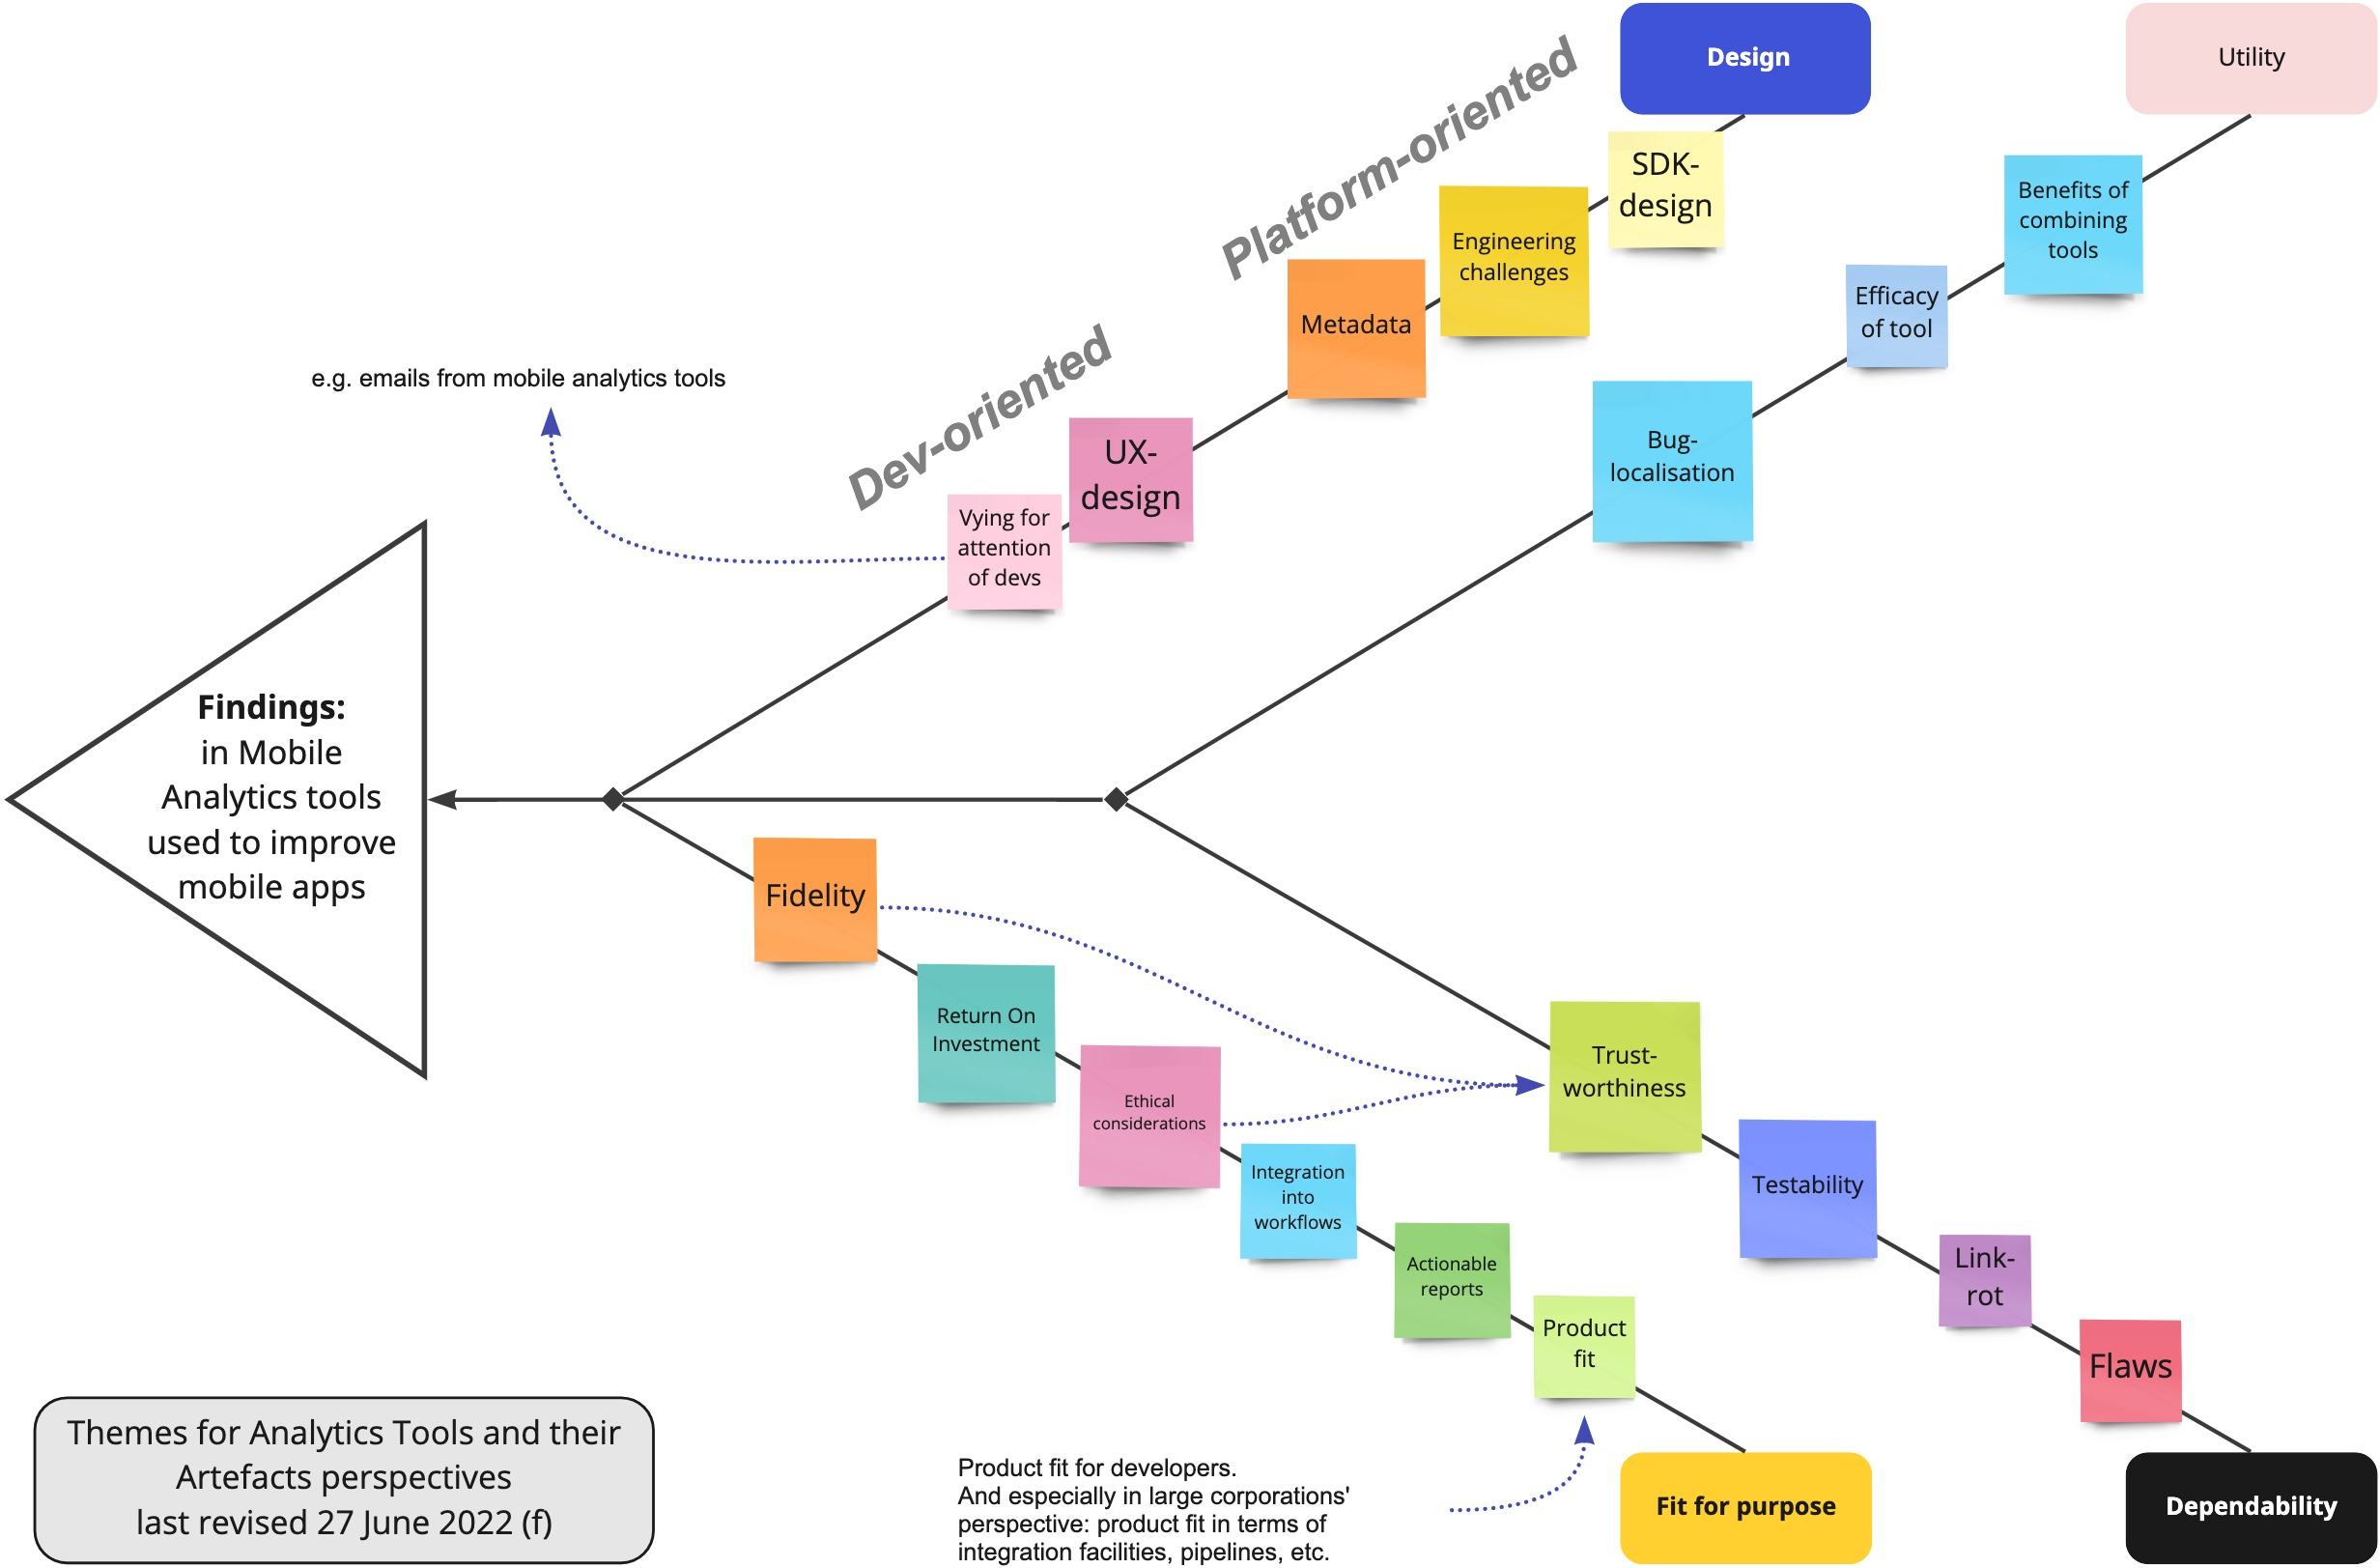
\includegraphics[width=\linewidth]{images/rough-sketches/analytics-tools-and-their-artefacts-fishbone-diagram-27-jun-2022f.jpeg}
    \caption{Analytics Tools and their Artefacts Fishbone Diagram\\Source: \href{https://miro.com/app/board/uXjVOtIsyWo=/?share_link_id=293061080490}{Miro}}
    \label{fig:analytics-tools-and-their-artefacts-fishbone-diagram}
\end{figure*}

\section{Design}~\label{tata-design-section}
Design emerged as by far the most pertinent topic for the mobile analytics tools. There are two key, connected facets: 


\begin{itemize}
\item the design of the on-device \Gls{sdk}, including addressing various engineering challenges and deciding on the meta-data to collect; and 
\item UX design to engage the developers to actually use the results of the mobile analytics [effectively].
\end{itemize}

The design of the on-device SDK is important because any in-app SDK needs to integrate easily in to the mobile app, and platform-level analytics need to be seamless and collect sufficient pertinent information to be useful for the app developers. They also need to be robust and timely in terms of collection, transmission, and processing of the underlying data in order for developers to have timely access to the results.

Mobile Analytics tools need to be used to be effective, and the user experience of the developers who use these tools where \emph{``developers’ needs are characterized by efficiency, informativeness, intuitiveness, and flexibility of the tool.''}~\sidecite[][p. 104]{kuusinen2016_flow_intrinsic_motivation_and_developer_experience_in_sw_eng}. Where using a tool is rewarding for the developers they are likely to use the tool more~\sidecite[][p. 260]{kuusinen2016_are_sw_devs_just_users_of_devt_tools_etc}.

These tools are a subset of software trying to get a developer's attention and they need to fit within a larger context. The tools need to surface (make visible) functionality and capabilities that align with the motivation(s) of the developers~\sidecite[][p. 2]{zaina2021_ux_information_in_the_daily_work_of_an_agile_team}.

\myindex{Fabric Crashlytics} is an archetypal example of how a mobile analytics tool can be designed to serve developers well. The product team developed it from the ground up, starting with excellent crash reporting, to provide developers with timely, actionable, attractive, and useful reports. This led to it becoming one of the top three mobile analytics tools for both iOS and Android within 10 months of being launched~\sidecite{___answersblog_2015_may_crashlytics-no1-in-performance}. % See also https://web.archive.org/web/20151203150947/http://fabric.io/blog/crashlytics-answers-named-top-mobile-sdks
First Twitter acquired it and then Google did; they subsequently integrated it into \myindex{Firebase Analytics} which is the most popular mobile analytics service for Android apps currently. 

It exemplified good design in terms of the SDK as it collected pertinent data developers found useful without requiring significant effort by the developers. The development team who created the SDK and the product had used their frustrations from using other analytics software as a catalyst to create Crashlytics. 

Similarly the user-interface of Crashlytics was slick from the outset and quickly adopted by app developers through presenting the analysis of the data the SDK had collected. It was designed from the outset to be actionable save \emph{`developers from information overload or ``analysis paralysis'''}~\sidecite{burke2014_wayne_chang_interview}.

Developers found it useful, it was free of charge, and the product continued to evolve and improve rapidly, for example by adding a general purpose mobile analytics service, called Answers, to Crashlytics that, in their words: \emph{``Before Answers, developers had to wade through mountains of data about their apps to find what they were looking for. We wanted to fix this, so we went to the drawing board and set out to build a mobile analytics solution you didn’t need to analyze.''}~\sidecite{___answersblog_2015_may_crashlytics-no1-in-performance} 

Platform-level analytics provides an outsider's perspective on the behaviour of mobile app, in contrast to in-app analytics that provides an insider's perspective. In this research Google's Android Vitals provides the platform-level analytics as it has the largest reach of any platform-level analytics across the widest range of devices. The platform provides users the ability to allow or deny analytics to be sent from their device. Apple's iOS (and MacOS) ask the user explicitly~\sidecite{apple_ios_share_diagnostics}, Android does not - users need to find the setting and opt-out~\sidecite{google_play_share_usage_and_diagnostics_info_with_google}. % See also https://chefkochblog.wordpress.com/2018/02/09/how-to-disable-android-usage-diagnostics-sharing/ I've not referenced this as they don't provide evidence of the default settings.

Mobile Analytics tools vie for attention against a plethora of other developer-oriented tools, project demands, \emph{etc.} Developers need to be enticed into using the tools and then retained on an ongoing basis to meet the objectives of the providers of the mobile analytics services.

\subsection{SDK design}~\label{section-sdk-design}
Any mobile analytics SDK needs to be designed to collect relevant data and forward that data so it can be processed, analysed, and reported on. The design of the client-side SDK affects many aspects of the data collection which then feeds subsequent stages in the processing of the data to provide the mobile analytics.

\newthought{Programming language support: } 
Mobile apps can be written in several programming languages, including Java, C++ and others. While many mobile apps are written in a single programming language some use several programming languages, for instance Kiwix Android combines Java, Kotlin, and C++. 
% More reading on Cordova's demise: https://medium.com/codex/the-sunset-of-apache-cordova-alternatives-for-cross-platform-mobile-development-in-2022-9da34234c992

Mobile analytics SDKs, in turn, support one or more of the programming languages. If they do not support the programming languages then they may not be able to obtain or provide analytics for elements written in the unsupported programming languages. For C and C++ code in particular, the app developers generally need to explicitly configure the code and the build process to incorporate the relevant mobile analytics SDK if it's available. % For a counterexample Fabric Crashlytics claimed their SDK was very easy to integrate https://web.archive.org/web/20151019132428/https://crashlytics.com/blog/the-wait-is-over-launching-crashlytics-for-android-ndk



\newthought{SDK initialisation: } 
The SDK needs to be initialised as early as practical each time the app is started (or restarted) if it's to capture pertinent information (including crashes that occur when the app starts or restarts): \emph{``for these products is that it would have to be wired in super early in the App's lifecycle, to (say) allow Crashlytics to capture crashes that happen early on''}~\sidecite[][issuecomment-635498836]{paularius2018_initialise_firebaseapp_without_google_services_json_issue_66}. 
% The discussion continued in https://github.com/firebase/firebase-android-sdk/issues/187 then returned to issue 66. And see also https://stackoverflow.com/questions/54927957/unable-to-make-firebase-work-for-a-non-gradle-build-missing-google-app-id-fire/55006495#55006495
For mobile analytics SDKs this has led to the developers of the SDK finding and implementing mechanisms to initialise their SDK in innovative (and unusual) ways, for instance Firebase uses a ContentProvider~\sidecite{stevenson2016_how_does_firebase_initialize_on_android}. Note: this does not always work, as reported in \sidecite{reddy2022_crashlytics_fails_to_track_app_startup_crashes}. When the SDK initialises it obtains various meta data about the app and the device. 
% \url{https://github.com/firebase/firebase-android-sdk/issues/66} % Found via https://lightrun.com/answers/firebase-firebase-android-sdk-initialize-firebaseapp-without-google-servicesjson

\newthought{Data automatically collected by SDKs: }
The mobile analytics SDKs have collected data automatically for years, the developers do not need to write additional code to collect this data. The data includes meta-data about the device and version of the platform. Depending on the SDK it may also collect demographic data, sensor data such as the geo-location, other data such as other apps that are installed, and various events that occur including network requests and responses. The data collected is covered shortly in \ref{section-meta-data}.

Any of these data elements \emph{may} help developers to improve their software, however, use of this data may be considered a privacy risk, particularly for end-users and may lead to ethical conundra for the development team and their organisation, see \ref{aiu-ethics-and-pii-topics}.

\newthought{Breadcrumbs: }
In 2015 HP's recently launched AppPulse Mobile SDK automatically instrumented a mobile app to. add crash reporting and the recording of screen transitions together with various meta-data. Both their iOS and Android \Glspl{sdk} provided similar capabilities in terms of an \Gls{api} developers could optionally call to record breadcrumbs in: Android~\sidecite{microfocus2018_apppulse_mobile_android_getting_started_video, hp_apppulse_mobile_android_guide_v1_9} and iOS~\sidecite{freeman2016_apppulse_ios_mobile_example}.

\newthought{Runtime activities for the SDK: } 
When the SDK is running, which they do in the background without being visible to the user of the app, they are responsible for the safekeeping and transmission of the collected data. Some collect data automatically, or autonomously. For example, Sentry's in-app SDK collects `automatic instrumentation'~\sidecite{sentry2021_mobile_vitals_four_metrics_every_mobile_developer_should_care_about}, and Android Vitals collects usage data, app crashes, and ANRs automatically.

At least some of the SDKs store analytics data locally on the device on an interim basis, the stored data would be removed once it had been successfully transmitted. Various SDKs limit the number of items they store. The SDKs also vary in how and when they transmit the data and on their behaviour if there isn't a suitable network connection to transmit the data.


\newthought{In-app analytics support for detecting ANRs: } 
At the start of the research in-app analytics SDKs were not able to measure ANRs which meant Android Vitals was the primary source of \Gls{anr} analytics for Android app developers. Subsequently, an opensource utility called \myindex{ANR watchdog} was released that uses a watchdog timer to detect ANRs~\sidecite{salomonbrys_github_anr_watchdog}. 
Investigating it in depth was beyond the scope of the immediate research, nonetheless Sentry used that code as a basis for their ANR reporting (\href{https://github.com/getsentry/sentry-java/blob/3f8d7b1cc869bb056c9db99b459e43f6c375784a/sentry-android-core/src/main/java/io/sentry/android/core/ANRWatchDog.java}{sentry-android-core...ANRWatchDog.java}). 

Note: Google has subsequently added a mechanism to enable apps to obtain information about previous ANRs when the app next started. The method is \index{getHistoricalProcessExitReasons}\href{https://developer.android.com/reference/kotlin/android/app/ActivityManager#gethistoricalprocessexitreasons}{\texttt{getHistoricalProcessExitReasons()}}~\sidenote{The source code is available online: \href{https://android.googlesource.com/platform/frameworks/base/+/master/core/java/android/app/ApplicationExitInfo.java}{android.googlesource.com/ ..... /ApplicationExitInfo.java} and provides more details of the design and the data structures.}, added in \href{https://developer.android.com/about/versions/11}{Android 11}, API level 30.
% Various discussions and explanations of using this API follow:
% https://commonsware.com/R/pages/chap-dataaccess-002.html - possibly the best and clearest code examples with explanations.
% Announcing the new functionality in 2021 https://firebase.blog/posts/2021/11/whats-new-at-Firebase-Summit-2021
% https://medium.com/@yangweigbh/monitoring-app-termination-on-android-11-97d514a3f9 
% Facebook's SDK to obtain cached ANRs https://developers.facebook.com/docs/reference/androidsdk/current/facebook/com/facebook/internal/instrument/anrreport/anrhandler.html/ and https://github.com/facebook/facebook-android-sdk/blob/5fe6e2a9d7056a17f54c1cae13e00788723d34f6/facebook-core/src/main/java/com/facebook/internal/instrument/anrreport/ANRHandler.kt
%
At the time of writing, Firebase Analytics uses this mechanism to obtain the \Gls{anr} and other app exit data~\sidenote{\href{https://github.com/firebase/firebase-android-sdk/blob/73131b69b0134456441e7fa218964b6a766fcec7/firebase-crashlytics/src/main/java/com/google/firebase/crashlytics/FirebaseCrashlytics.java}{github.com ..... FirebaseCrashlytics.java}}.


\subsubsection{Runtime encapsulation of failures}~\label{tata-runtime-encapsulation-of-errors}
\newthought{Limitations in visibility by an SDK: } 
In short, the viewpoint of the SDK affects and can limit what it can observe/record. Also some mobile apps incorporate their own runtime which may hide some failures from being observed by the platform.

\newthought{Android Vitals: } 
Android Vitals does not collect crashes that are contained within an application's runtime. React-Native is a popular cross-platform app development framework. It includes its own application runtime environment and this runtime automatically restarts the app if it crashes. These crashes are not visible to Android Vitals as evidenced by two of the apps within the app centric case studies -- \myindex{LocalHalo} and \Gls{gtaf}'s Taskinator app\index{GTAF} -- where Android Vitals showed no crashes for either of these apps, with one exception. 

The LocalHalo app-centric case study provides an illustration where app crashes were not observed by Android Vitals until a failure in the React Native runtime occurred.

% The following is hacked it should dynamically calculate the width of the full page (\textwidth is calculated earlier and doesn't account for the extra width provided by using figure* I have read about how to address this for captions (see https://tex.stackexchange.com/a/128490/88466), for now I'll live with the hack.
\begin{figure*}[htbp!]
\RawFloats
\centering
\begin{minipage}{.45\linewidth}
  \centering
  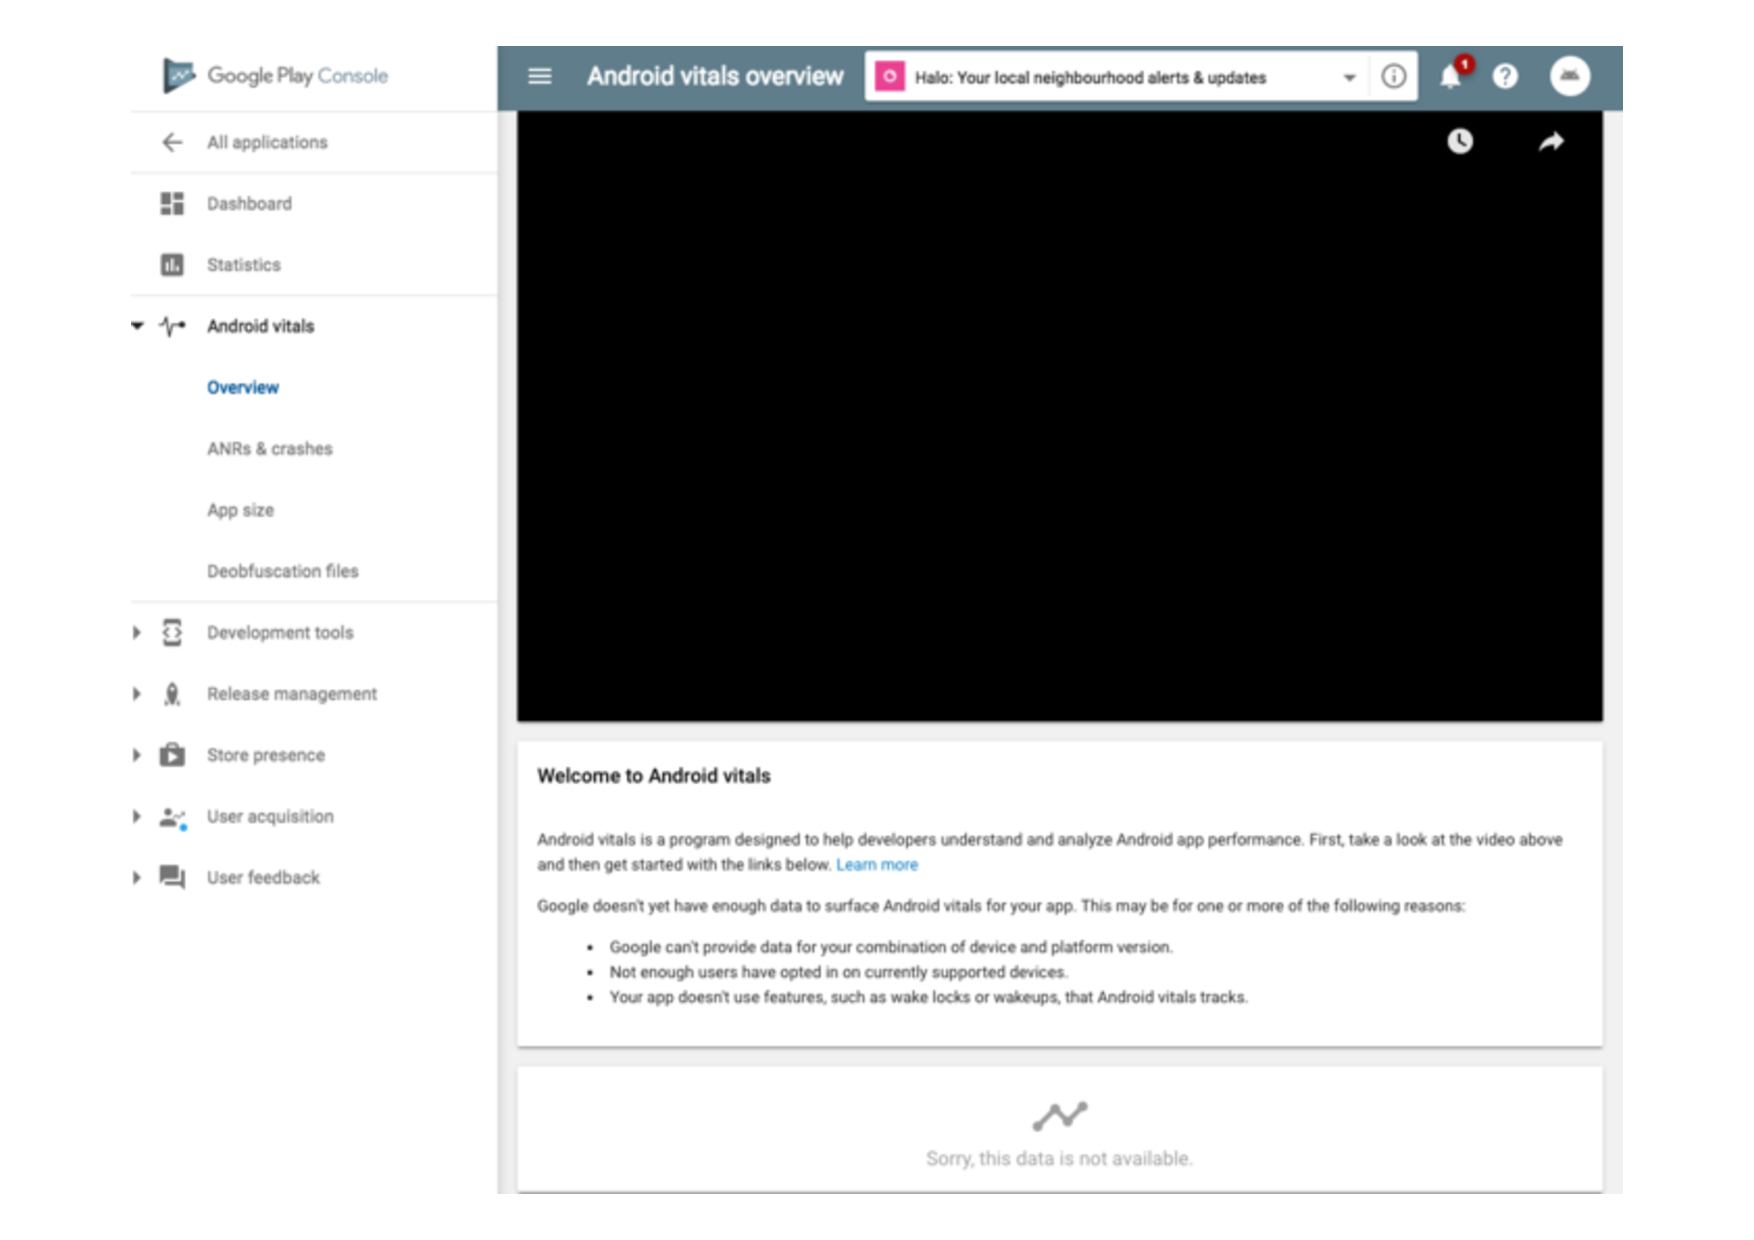
\includegraphics[width=\linewidth]{images/localhalo/apphealthoverviewplace_5550596_no_data.pdf}
  \captionof*{figure}{App Health Overview page}
\end{minipage}\hfill%
\begin{minipage}{.45\linewidth}
  \centering
  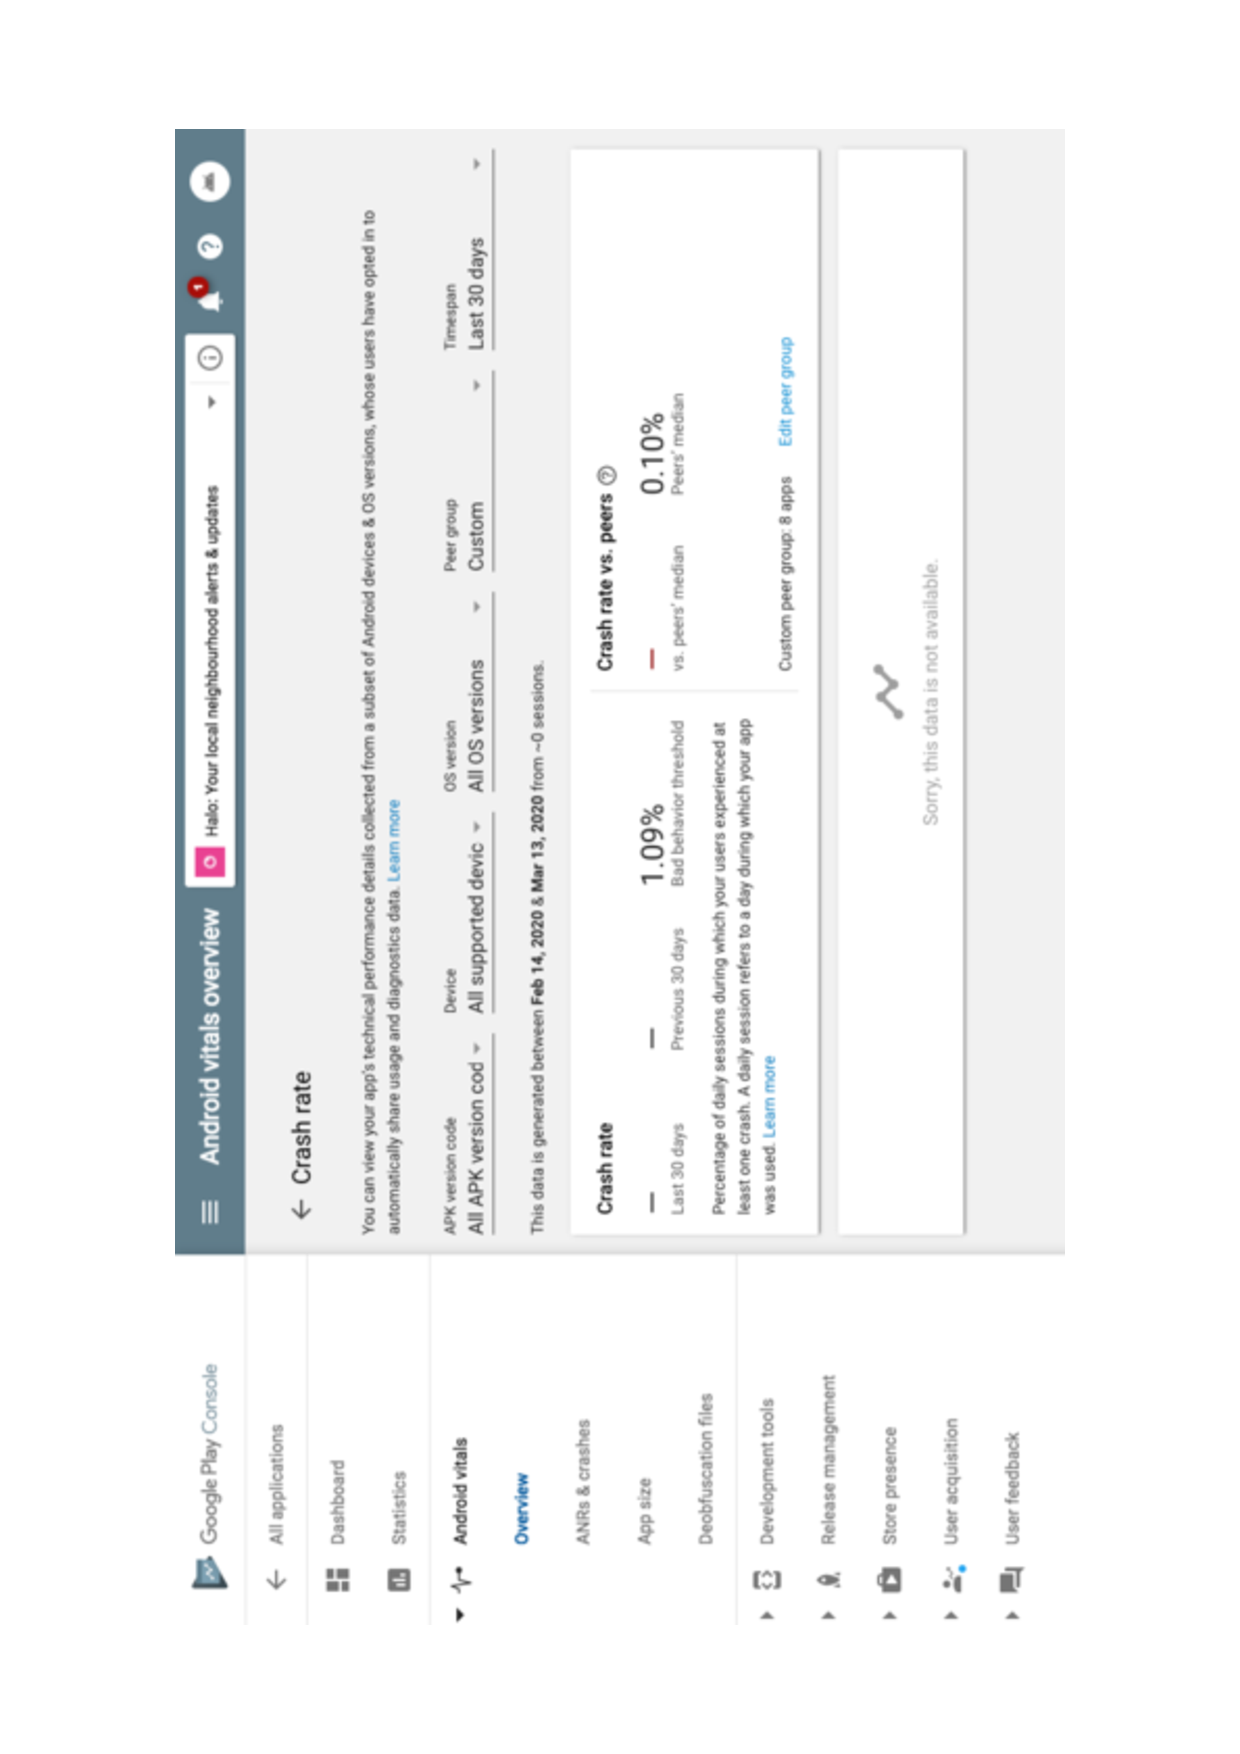
\includegraphics[width=\linewidth]{images/localhalo/apphealthdetailsplace_55505963_no_data.pdf}
  \captionof*{figure}{App Health Details page}
\end{minipage}
    \caption{No Android Vitals reports on \nth{16} March 2020}
    \label{fig:localhalo-android-vitals-no-data-16-march-2020}
\end{figure*}

Figure~\ref{fig:localhalo-android-vitals-high-failures-26-march-2020} was recorded ten days later in \nth{26} March 2020 and shows the alerts for both high crash and ANR rates in the App Health Overview page and the graph for the rampant crash rate in the corresponding App Health Details page. These indicate the failures were related to the native runtime rather than within the React Native code. These were not reported by any Sentry Alerts and they do not appear in the weekly summary reports, except potentially by the absence of data shown in Figure~\ref{fig:sentry-missing-data-march-2020}. While the reason for this was not explained in the interviews or in the analytics data, it is likely that this caused by severe crashes that prevented Sentry's SDK from reporting any data.

\begin{figure*}[htbp!]
\RawFloats
\centering
\begin{minipage}{.45\linewidth}
  \centering
  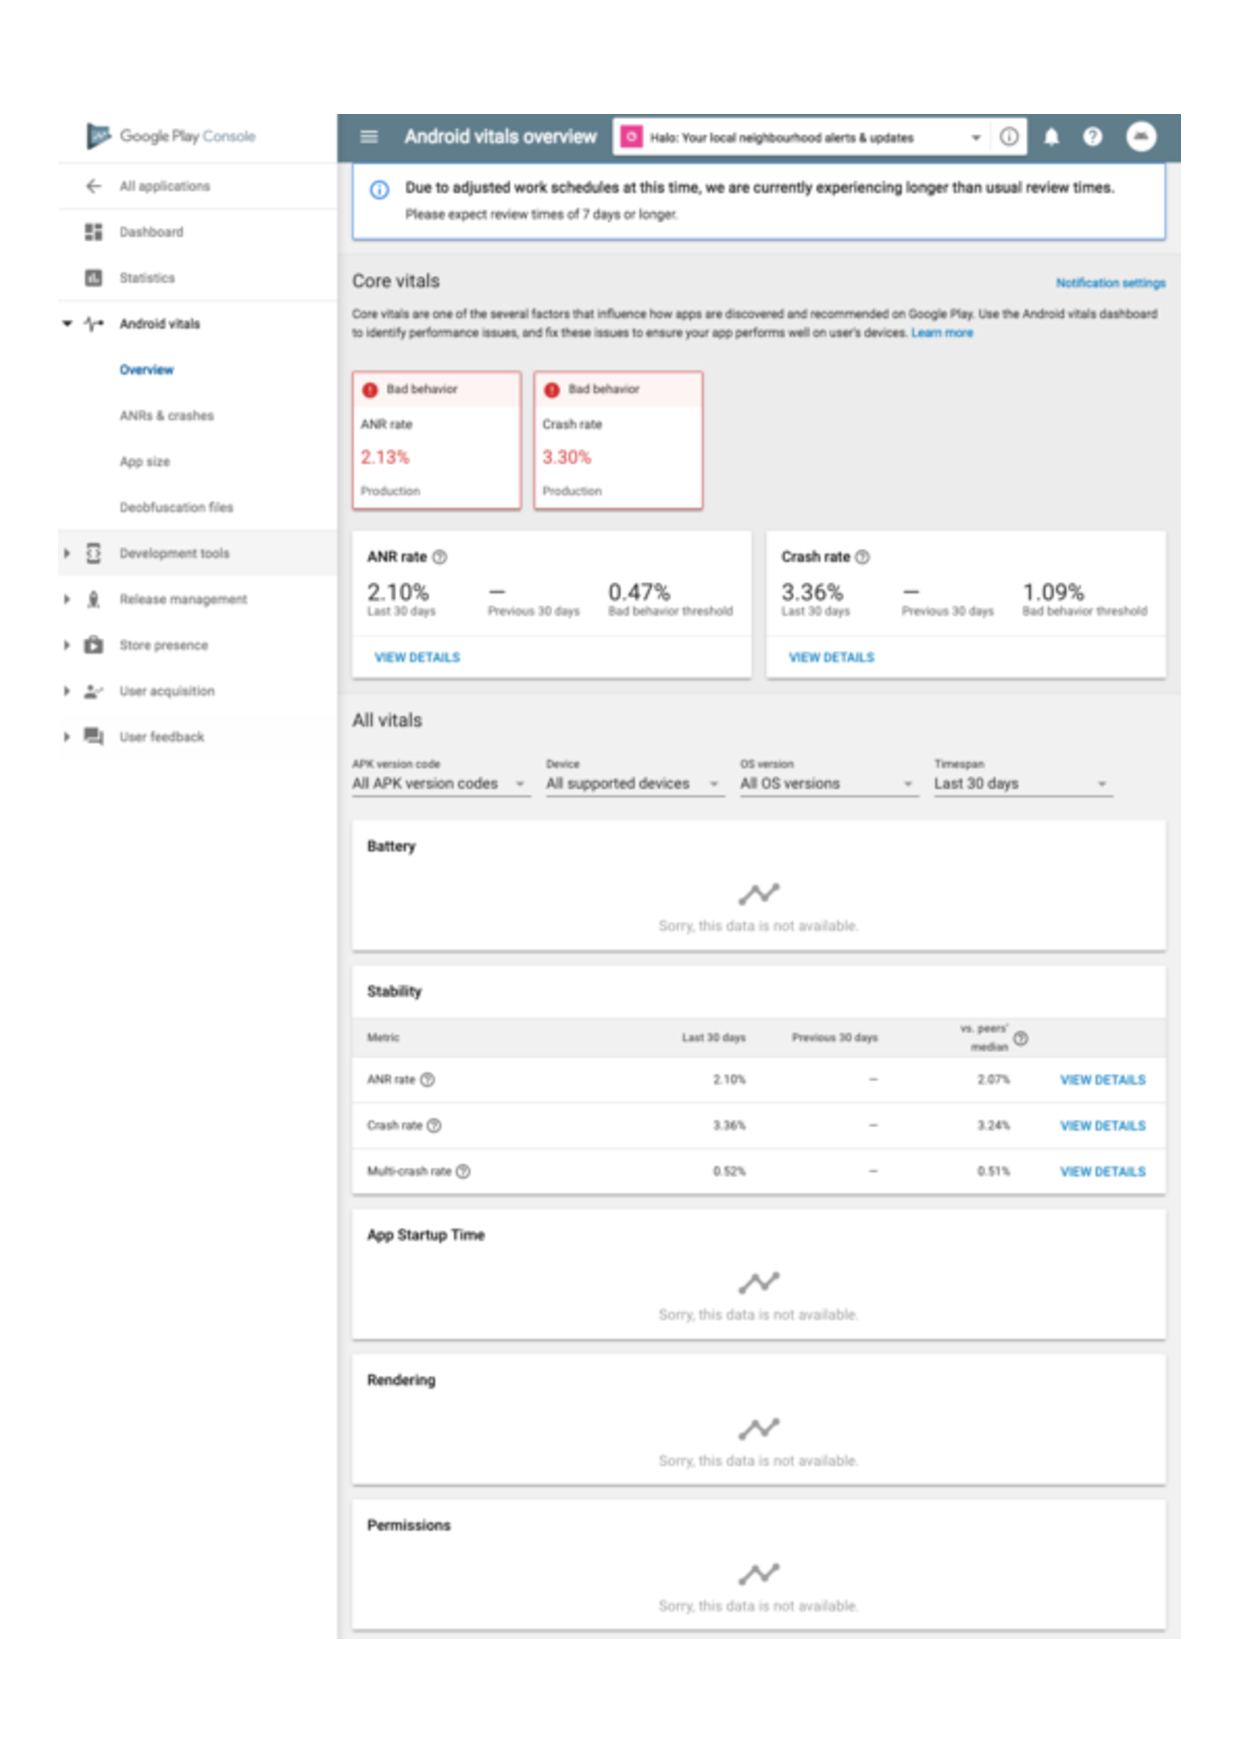
\includegraphics[width=\linewidth]{images/localhalo/apphealthoverviewplace_5550596_high_errors.pdf}
  \captionof*{figure}{App Health Overview page}
\end{minipage}\hfill%
\begin{minipage}{.45\linewidth}
  \centering
  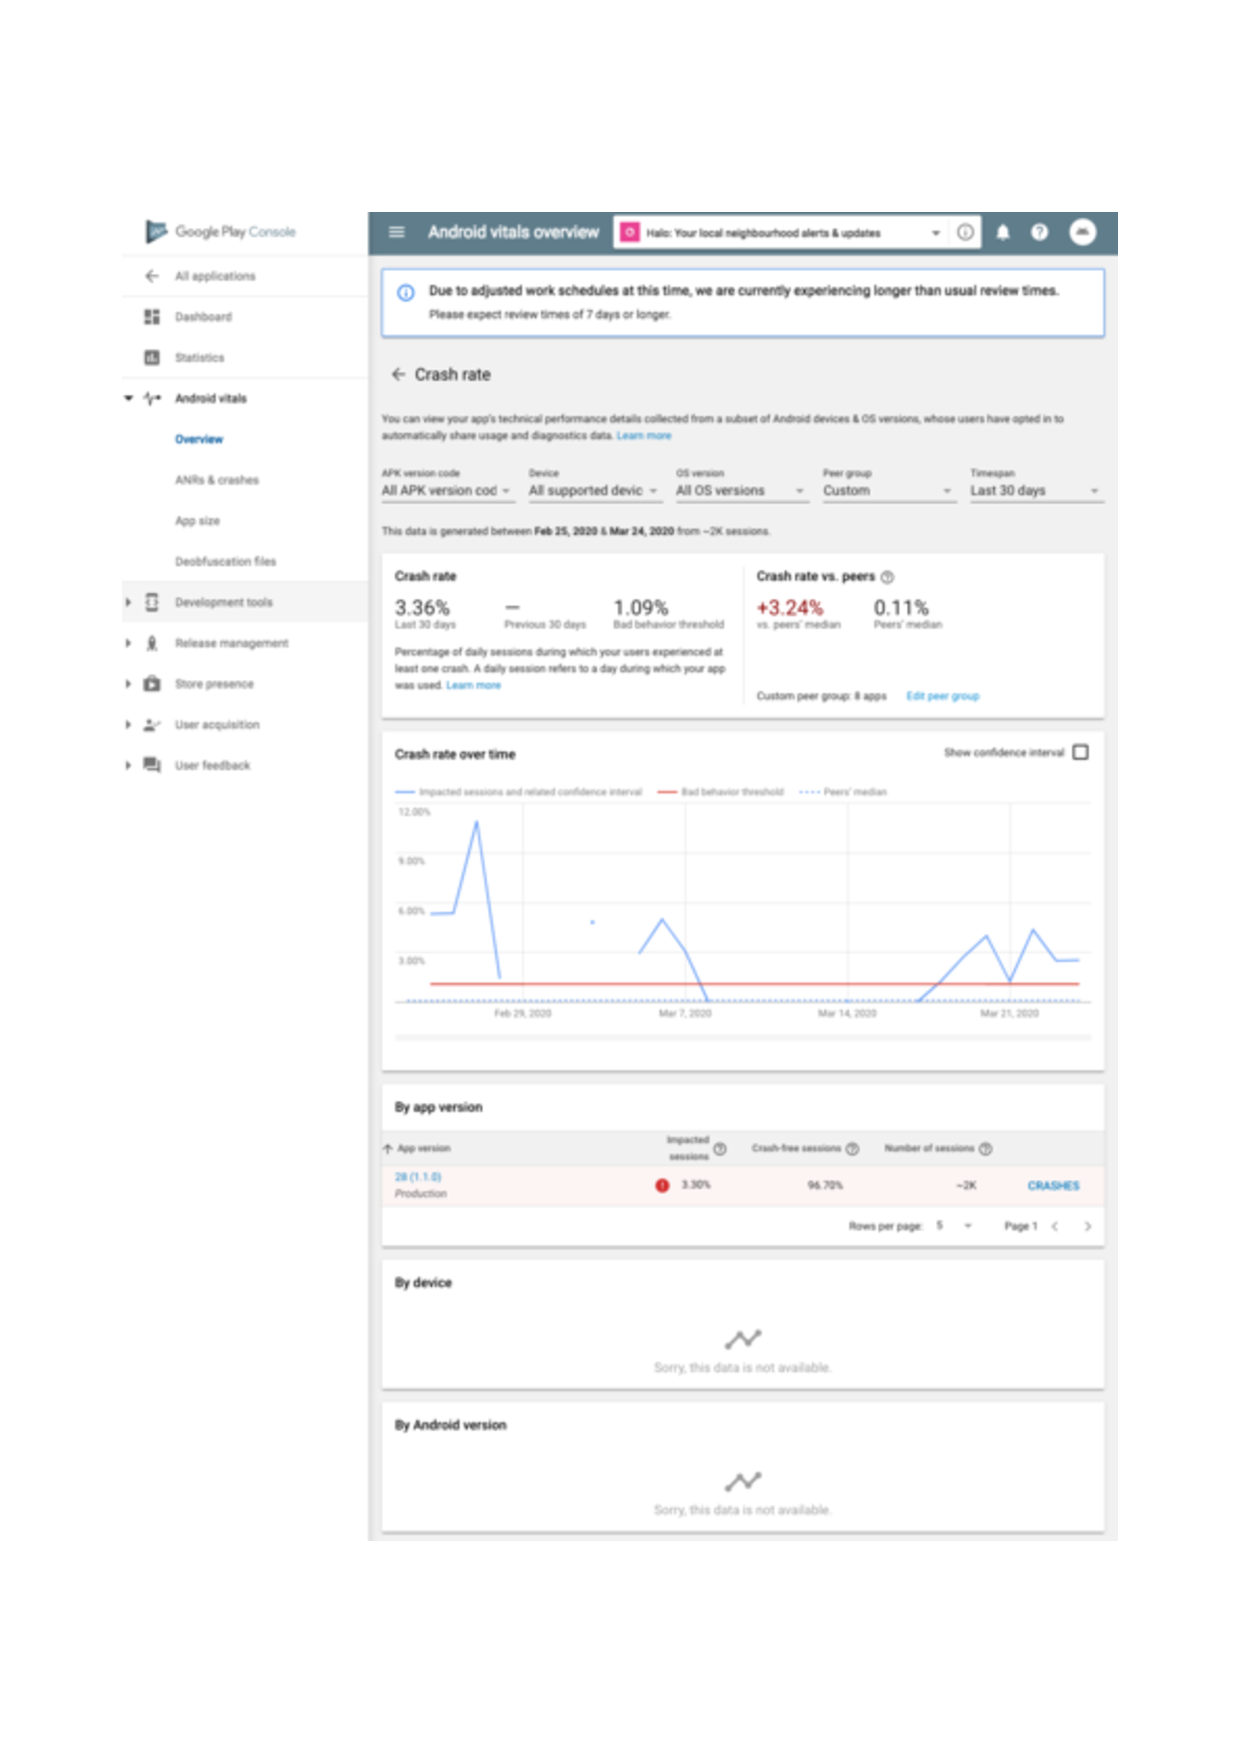
\includegraphics[width=\linewidth]{images/localhalo/apphealthdetailsplace_55505963_high_errors.pdf}
  \captionof*{figure}{App Health Details page}
\end{minipage}
    \caption{Alerts and graphs in Android Vitals on \nth{26} March 2020}
    \label{fig:localhalo-android-vitals-high-failures-26-march-2020}
\end{figure*}

A release in March 2020 had a high crash rate for the production release of their Android app. The top crash cluster was for:

{\small \texttt{java.lang.RuntimeExceptionhost.exp.exponent.experience.a\$b.run}} 

This was traced to a problem in the expo library the development team used in the app~\sidecite{expo2019_issue5839}~\footnote{Expo is a very popular open source platform for making universal native apps that run on Android, iOS, and the web \url{https://github.com/expo/expo}.}. In that issue, several developers for different Android apps provide data from Google Play Console confirming they also receive similar crash clusters. The cause has not yet been definitively traced or addressed, however for the LocalHalo app the crashes stopped being reported once a new release (1.3.0) of the Android app, was launched around \nth{6} April 2020.


\begin{figure*}[htbp!]
\RawFloats
\centering
\begin{minipage}{.45\textwidth}
  \centering
  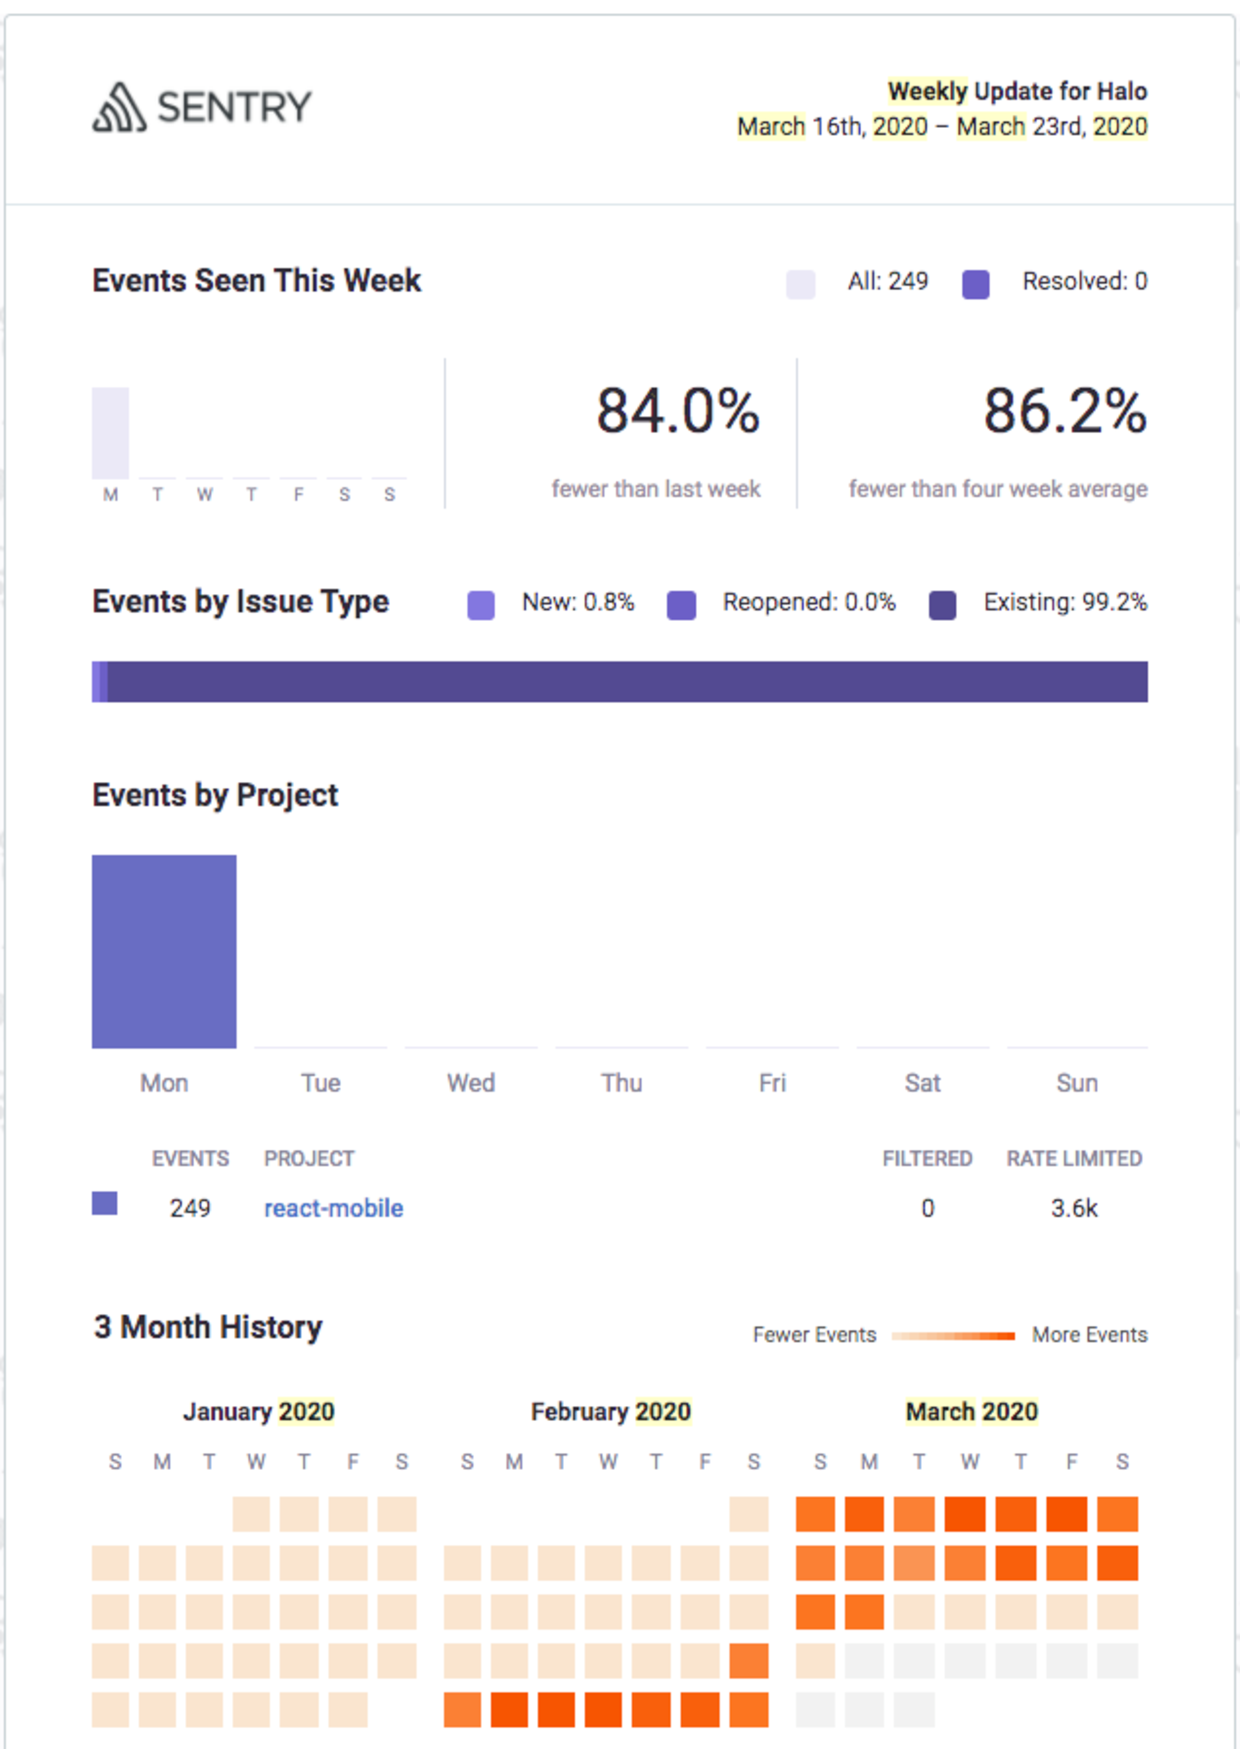
\includegraphics[width=\textwidth]{images/localhalo/sentry-weekly-report-16-mar-2020.pdf}
  \captionof*{figure}{\nth{16} -~\nth{22} March 2020}
  \label{fig:localhalo-sentry-weekly-report-16-mar-2020}
\end{minipage}\hfill%
\begin{minipage}{.45\textwidth}
  \centering
  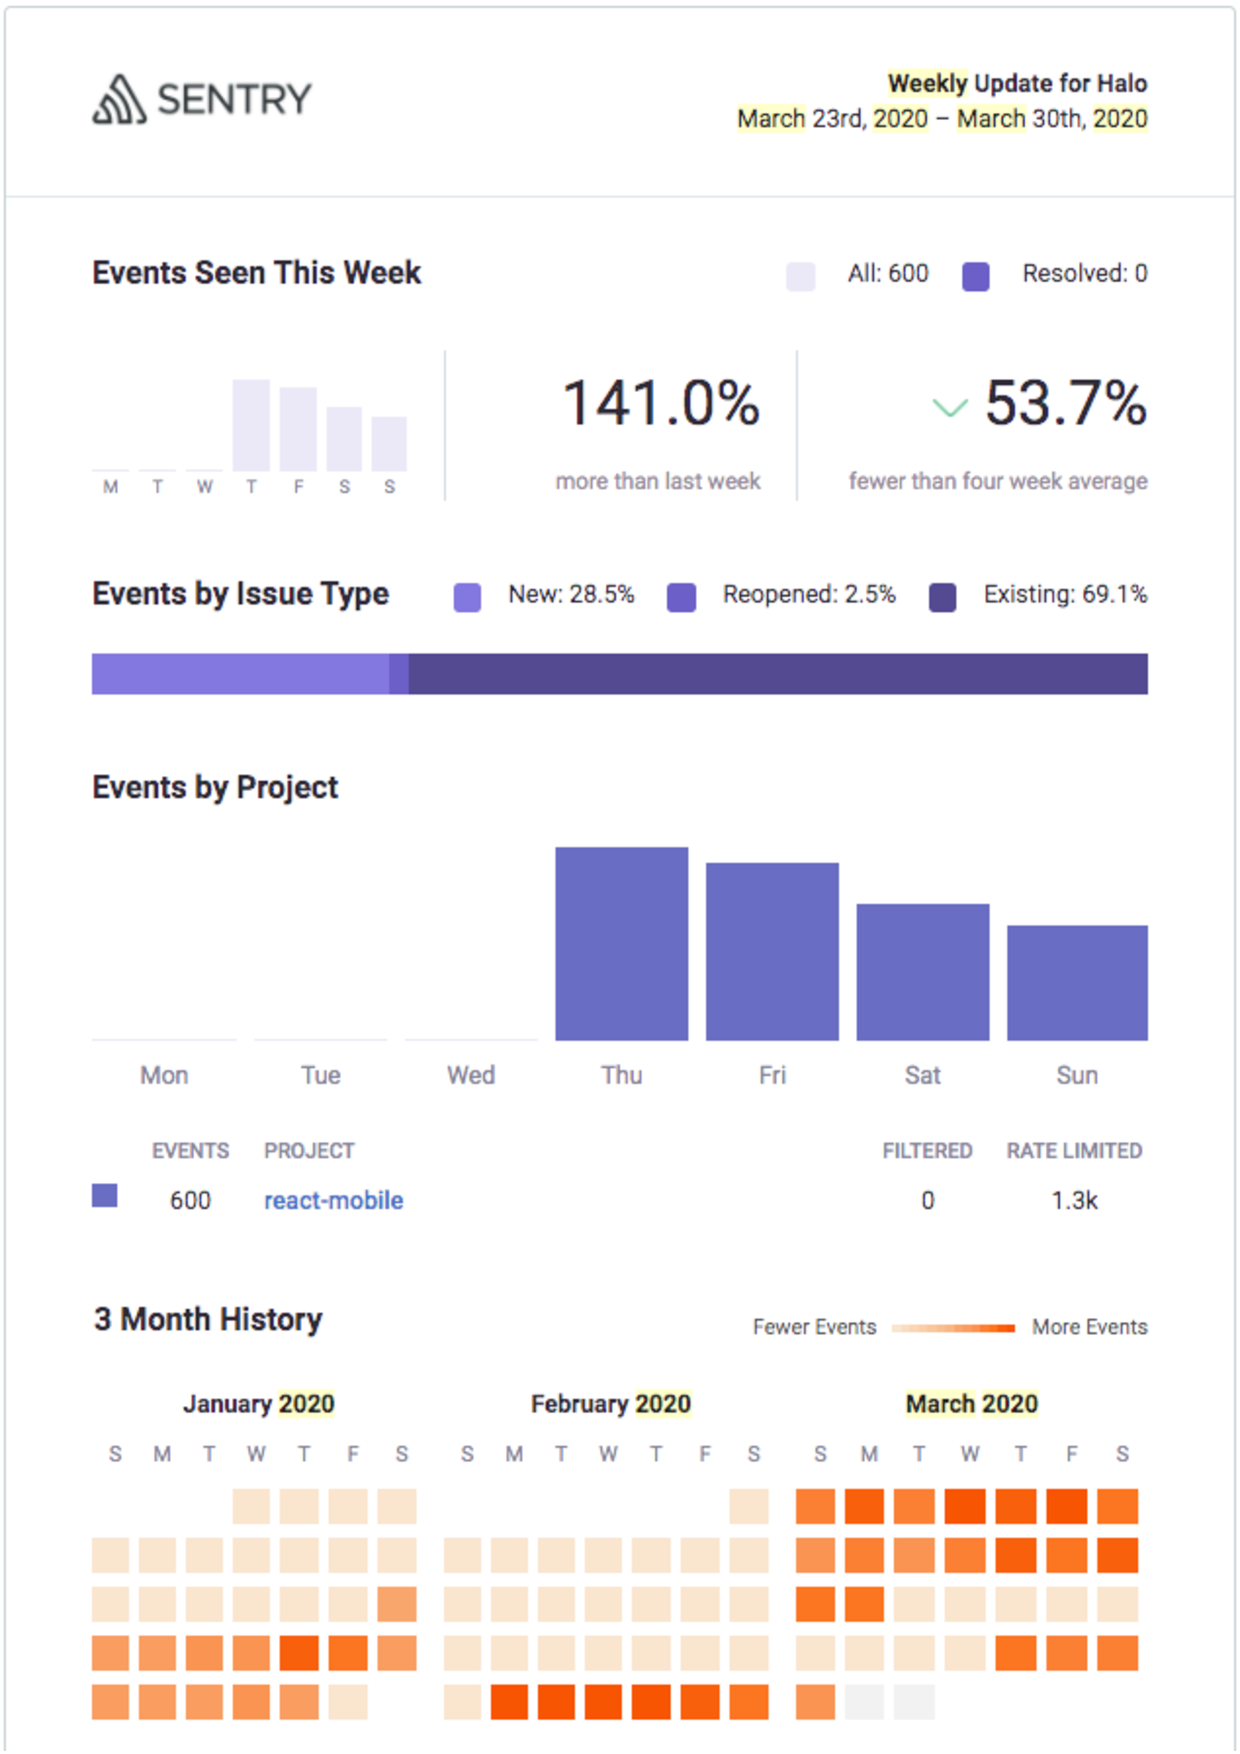
\includegraphics[width=\textwidth]{images/localhalo/sentry-weekly-report-23-mar-2020.pdf}
  \captionof*{figure}{\nth{23} -~\nth{29} March 2020}
  \label{fig:localhalo-sentry-weekly-report-23-mar-2020}
\end{minipage}
    \caption{Missing data reported in Sentry, in March 2020}
    \label{fig:sentry-missing-data-march-2020}
\end{figure*}

\newthought{Some failures did emerge when the runtime encapsulation fails: }
That exception was when Android Vitals did report crashes in March and April 2020. Figure \ref{fig:localhalo-android-vitals-no-data-16-march-2020} was recorded on \nth{16} March 2020 before these started and shows the App Health Overview page with a link to a video introducing Android Vitals~\sidenote{This appears as a mainly black rectangle in this thumbnail screenshot.}, and the App Health Details page with no data.

\subsubsection{Meta-data}~\label{section-meta-data}
Meta-data is not about the app \emph{per se}, but about the user and/or the user's device, \emph{etc.} 
Meta-data may help developers with bug localisation and reproduction pertaining to the device model, its underlying hardware characteristics, the release of the platform, and so on. 

Figure \ref{fig:fabric-crashlytics-privacy-policy} provides an illustration of the privacy policy for Fabric Crashlytics which lists various the meta-data it collected at the time. The successor Firebase Crashlytics lists similar data being collected for crashes~\url{https://firebase.google.com/support/privacy#crash-stored-info}. The details of why these details were necessary was discussed online by \href{https://stackoverflow.com/users/3975963/mike-bonnell}{Mike Bonnell}, 
one of the Crashlytics engineering team, in response to a question on StackOverflow~\sidecite{kim2017_what_information_does_crashlytics_collect_from_end_users}.

\begin{figure}
    \centering
    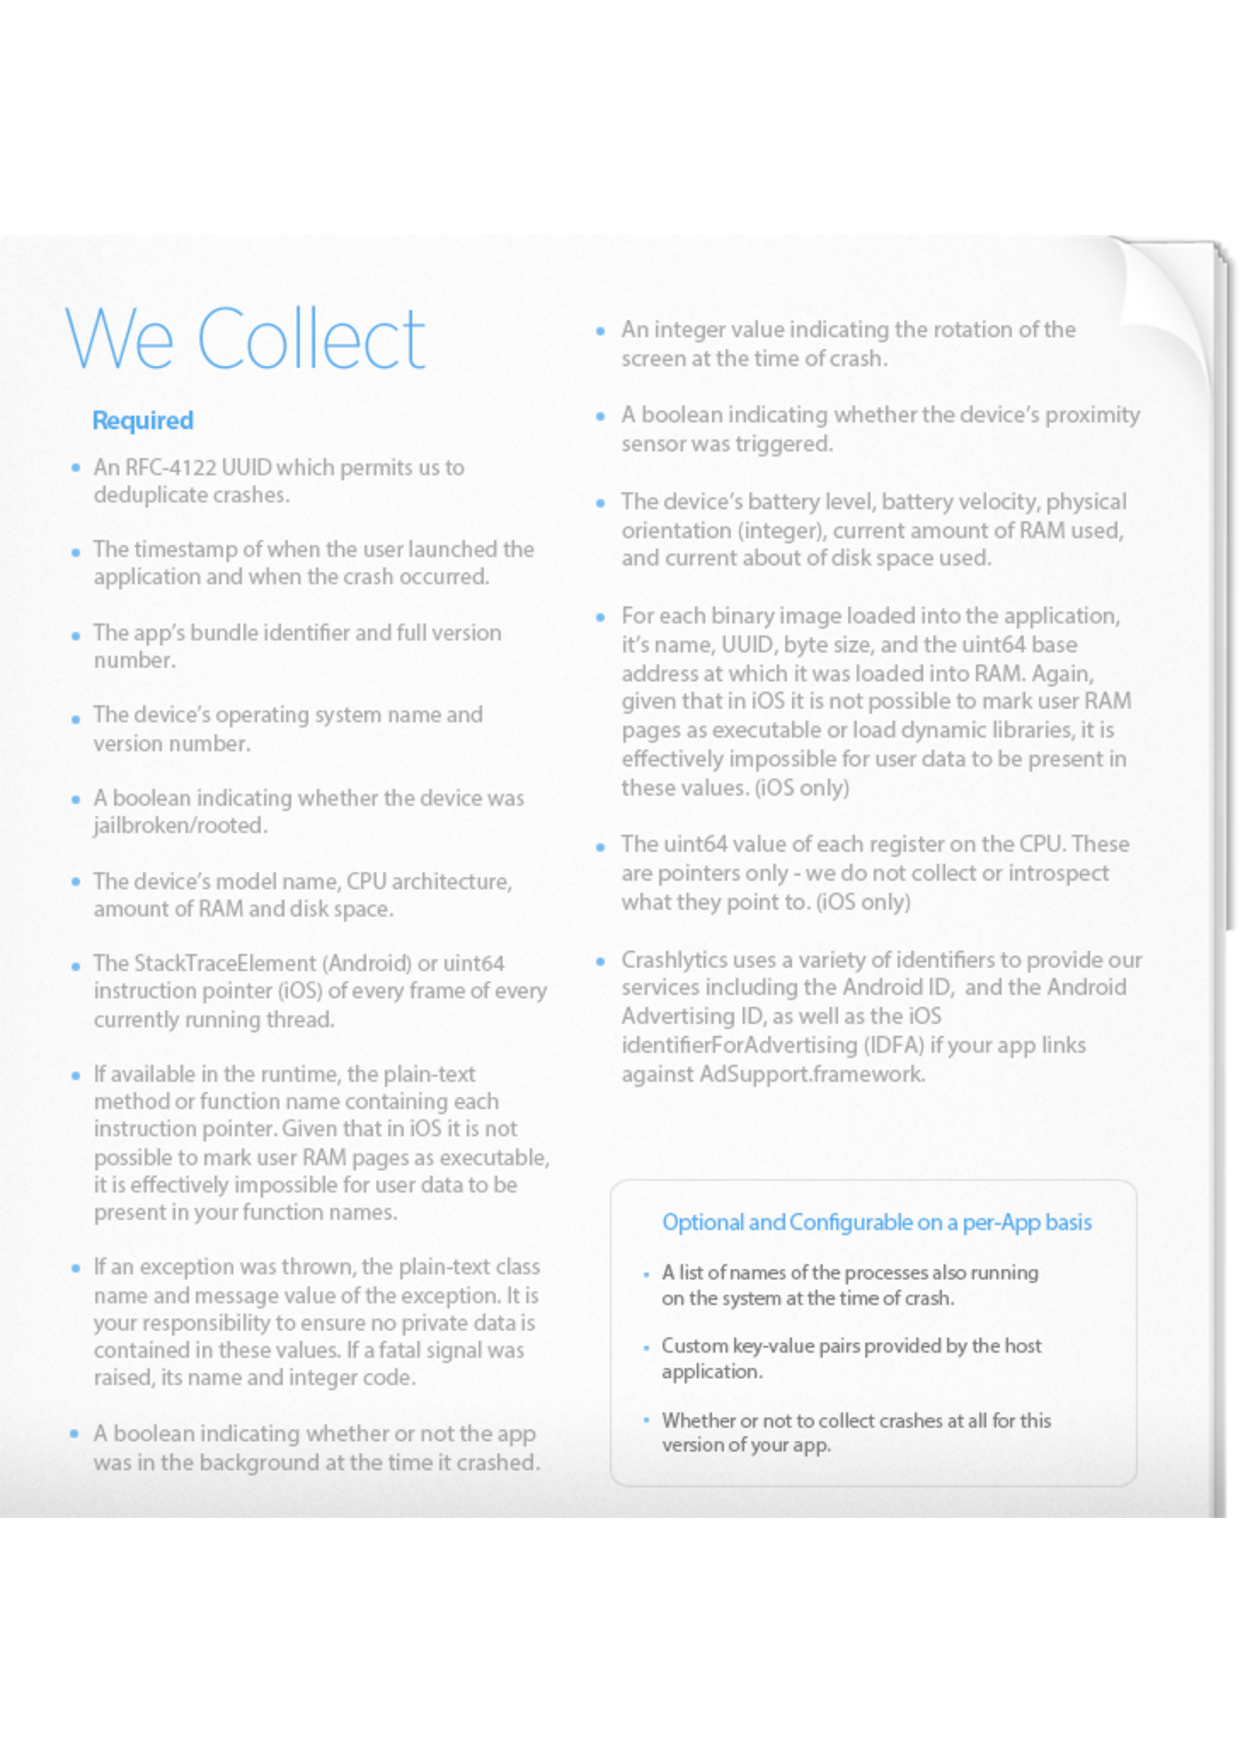
\includegraphics[width=10cm]{images/fabric-crashlytics/crashlytics-privacy-policy-38154ffbd69ef44a478b54365dc9b3ad.pdf}
    \caption[Fabric Crashlytics Privacy Policy (in 2015)]{Fabric Crashlytics Privacy Policy (in 2015)\\{source: \tiny \url{https://web.archive.org/web/20150405071731/http://try.crashlytics.com/security/}}}
    \label{fig:fabric-crashlytics-privacy-policy}
\end{figure}

Of note, some app developers may receive data they didn't expect, particularly if they migrated from \myindex{Fabric Crashlytics} to \myindex{Firebase Crashlytics}. 

To provide some additional context Fabric and Firebase both offered facilities to combine various datasets into their reporting, for instance based on advertising SDKs. This led to reports that included demographics in addition to the crash analytics, \emph{etc.}~\footnote{Discussions on how the demographics are captured and made available include~\cite{joe2016_firebase_analytics_demographics} and~\cite{chelo2020_firebase_does_not_collect_age_or_gender_data}.}. 

The forced migration from Fabric Crashlytics to Firebase Crashlytics had two stages, the first was to migrate the project to the Firebase user interface and the second was to replace the Fabric SDK with the Firebase SDK. The Firebase SDK automatically collected additional data~\sidecite{firebase_help_GA4_2021_predefined_user_dimensions}.


As mentioned in \secref{aata-tradeoffs-topic}, the Catrobat project chose to stop using Firebase Crashlytics when they discovered that the demographics of the end users were also being recorded. 

In collaborative research into using Firebase Analytics for logging, 50 of 107 active Android opensource projects initialised just the Firebase Analytics SDK; they did not use any other aspect of the SDK~\sidecite{harty2021_logging_practices_with_mobile_analytics}~\sidenote{Perhaps they thought that `Getting Started' was all they needed to do? or perhaps the default data was `good enough'?}. Therefore the contents and the limitations of the default meta-data are of particular interest, since default meta-data is all those developers would have available to them. The remaining 57 projects used additional API calls to record additional information on one or more code-paths in the respective app.

\subsubsection{Engineering challenges}~\label{section-engineering-challenges}
Engineering challenges relate to developing the components of the mobile analytics tool/service such as provision of a client-side SDK that collects failures for native (C++) code.

Engineering challenges for mobile analytics include:
\begin{itemize}
    \item Support for collecting information from native code. This can be particularly pertinent for apps that include libraries in native code that are provided by third-parties.
    \item Collecting information from the earliest stage of app startup to the app's shutdown; otherwise data collection is incomplete.
    \item Establishing and maintaining sufficient information to calculate and provide sufficiently accurate comparisons, ratios, and so on. As an example, determining the Probability of Failure On Demand (\href{glossary-pfod}{PFOD}), requires counts of non-failures -- those events/transactions/\emph{etc.} that \emph{worked}. Also, the sources/inputs/conditions that contributed to the failure may be useful to the app developer; does the mobile analytics SDK collect these? In the \myindex{Kiwix} case study; there were various sources of WebView crashes, these needed to be identified in order to attempt to prevent similar crashes in future.
    \item For the Vitals Scraper utility developed as part of this research, there were engineering challenges in first developing and then maintaining an automated interface to obtain reports and related information from Google Play Console and Android Vitals.
    \item For platform tools, collecting pertinent information across the process boundary includes engineering challenges. For in-app analytics, collecting information, such as ANRs, was a challenge during the period of the active app-centric case studies. 
\end{itemize}

These challenges are ongoing, various \Glspl{sdk} aim to address one or more of them.

\subsection{Developer experience}~\label{tata-developer-experience-ux-design}
The design of the User Experience (UX) of the mobile analytics tool for their audience of the software development team (and particularly the app developers).

% TODO add examples from the case-studies

\newthought{Vying for the attention of developers: }
Mobile Analytics tools compete for finite attention developers are able to provide. This competition occurs at the initial selection and integration phases and continues during the life of the app. This includes seeing attention on an ongoing basis  to communicate their alerts, reports, \emph{etc.} Pricing, licensing, and management approvals sometimes prevent some development team members from being able to use the tools directly.

\begin{itemize}
    \itemsep0em
    \item Access and use of mobile analytics tools allows them to be used interactively, where this is impractical copies, extracts, \emph{etc.} of reports and related material helps  preserve them for future analysis, for evidence, and so on. These copies and extracts can also extend the reach to people who don't have direct access to the tools. Several of the app-centric case studies, including Kiwix, Catrobat, LocalHalo, and the Commercial project limited access to various tools to a subset of the developers. In contrast, Moonpig, provided access to every member of the development team who had access to the source code of the app.
    \item When the analytics tools lack the attention of developers the effects of existing and new issues propagate and may enable these issues to snowball. The Kiwix project provided a good example of this with the loss of the lead developer for the Android app.
    \item The majority of the app-centric case studies used multiple mobile analytic tools. Some of the developers chose to ignore aspects of particular tools, for instance the crash analytics in Android Vitals in favour for similar services from other tools, even though Android Vitals is able to record some crashes that the other tools do not capture \emph{e.g.} owing to limitations in the respective SDK. The tools need to convince developers of the merits of their reports. The Moonpig development team, in particular, checked the reports of multiple tools to reduce their blind-spots.
    \item The LocalHalo project illustrated the flip-flop of failures between two analytics tools. This was insightful and demonstrates the value of having a combination of platform-level and in-app analytics, at least for apps written in frameworks such as react-native.
\end{itemize}

\newthought{Design of the mobile analytics events and content: }
\hypertarget{tata-design-of-mobile-analytics-events-and-content}{Of all} the mobile analytics tools covered in this research \myindex{Iteratively} uniquely focused on the design and verification that the mobile analytics captured the intended data. Their various software tools helped the teams design and implement the desired mobile analytics correctly in a mobile app.

\begin{kaobox}[frametitle=Industrial example of a major disconnect between perception and reality]
In my industry experience, not otherwise covered in my research, I discovered a profound disconnect between what the engineering leadership \emph{said} the mobile analytics collected, compared to what it \emph{actually} collected in the mobile app. Over 90\% of the claimed events were not implemented in the app. Had that project used tools such as those provided by Iteratively, the mismatch would have been identified by the software tools and clearly presented. Furthermore the client-side tooling Iteratively provided was able to fail the build of the app. 
\end{kaobox}

\section{Fitness-for-purpose}~\label{tata-fitness-for-purpose-section}
Simply put, the mobile analytics tools need to be fit for purpose. In the context of this research, fit for purpose means that the tools need to:\todo{Revisit the following list once I've added the subsections.}

\begin{itemize}
\item fit the needs and desires of the developers (product fit); 
\item provide actionable reports; and 
\item be a good return on any investment the developers make in terms of using the tools.
\end{itemize}
 
When the tools integrate into the workflows of the developers, they're more likely to be adopted as long-term companions and therefore demonstrate they provide a good return on investment. 

Note: two of the topics: fidelity and ethical considerations bridge both this section: fitness-for-purpose and the dependability section, they are covered in \secref{tata-cross-cutting-concerns}.

{\small
\begin{itemize}
    \itemsep0em
    \item \sout{Product Fit: whether, and if practical how well, the mobile analytics product fits the desires/needs of the developers and their organisation.}
    \item \sout{Actionable Reports: reports the developers can action in order to address concerns presented in the reports.}
    \item \sout{Integration into workflows: the ability of a given mobile analytics tool/service to be integrated into development team's workflows.}
    \item ROI (return-on-investment): developers may make both implicit and explicit choices on what to invest in, for instance in terms of their focus, their effort, and their money. The analytics tools need to convince developers a) to invest and then b) whether to increase that investment (and if so what forms of investment e.g. in terms of writing more code, spending [more] money, using the tool more, etc.).
\end{itemize}
}

\subsection{Product Fit}
\newthought{Product fit: } addresses whether, and if practical how well, the mobile analytics product fits the desires/needs of the developers and their organisation. It is similar, but more specific than product/market fit~\footnote{\url{https://en.wikipedia.org/wiki/Product/market_fit}} - or conversely the market is pico-sized, gauged at the level of a development team. % See also concepts from https://en.wikipedia.org/wiki/Lean_startup e.g. actionable metrics.

Developers of mobile analytics tools, such as Iteratively~\sidenote{Iteratively was acquired by Amplitude in 2021 and the products have been enhanced and integrated into Amplitude's product suite.}, seek ways to identify and determine what app developers will find useful. 

In interviews with Iteratively's CEO, he explained they used various techniques including `ten dots', illustrated in Figure \ref{fig:iteratively-product-market-fit}, during one-to-one semi-structured interviews to help Iteratively prioritise the features they developed and provided. Each interviewee was given the opportunity to complete this exercise, an example of their `dot-voting'~\sidecite{18f_dot_voting} is also provided in Figure \ref{fig:iteratively-product-market-fit}.
The CEO provided access to their live document containing the results of the `dot-voting' and gave permission to analyse it.~\todo{Consider whether to include the analysis of the dot-votes (currently in the relevant empirical studies chapter).}


\begin{figure}[htbp!]
\RawFloats
\centering
\begin{minipage}{.45\textwidth}
  \centering
  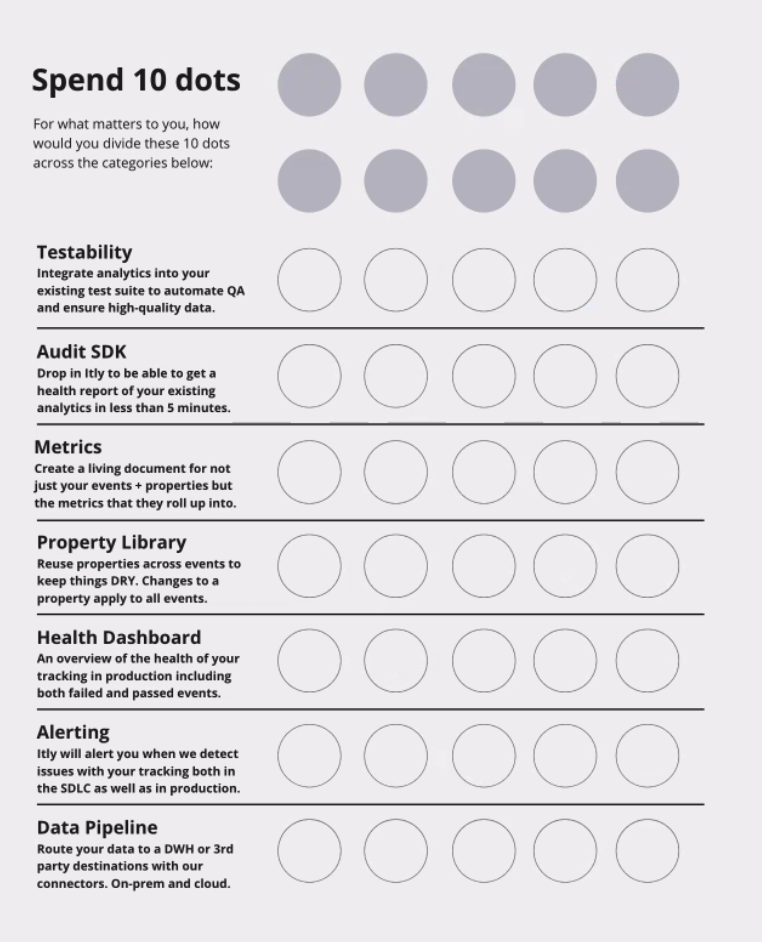
\includegraphics[width=\textwidth]{images/iteratively/spend-10-dots.png}
  \captionof*{figure}{Spend ten dots}
  \label{fig:iteratively-spend-ten-dots}
\end{minipage}\hfill%
\begin{minipage}{.45\textwidth}
  \centering
  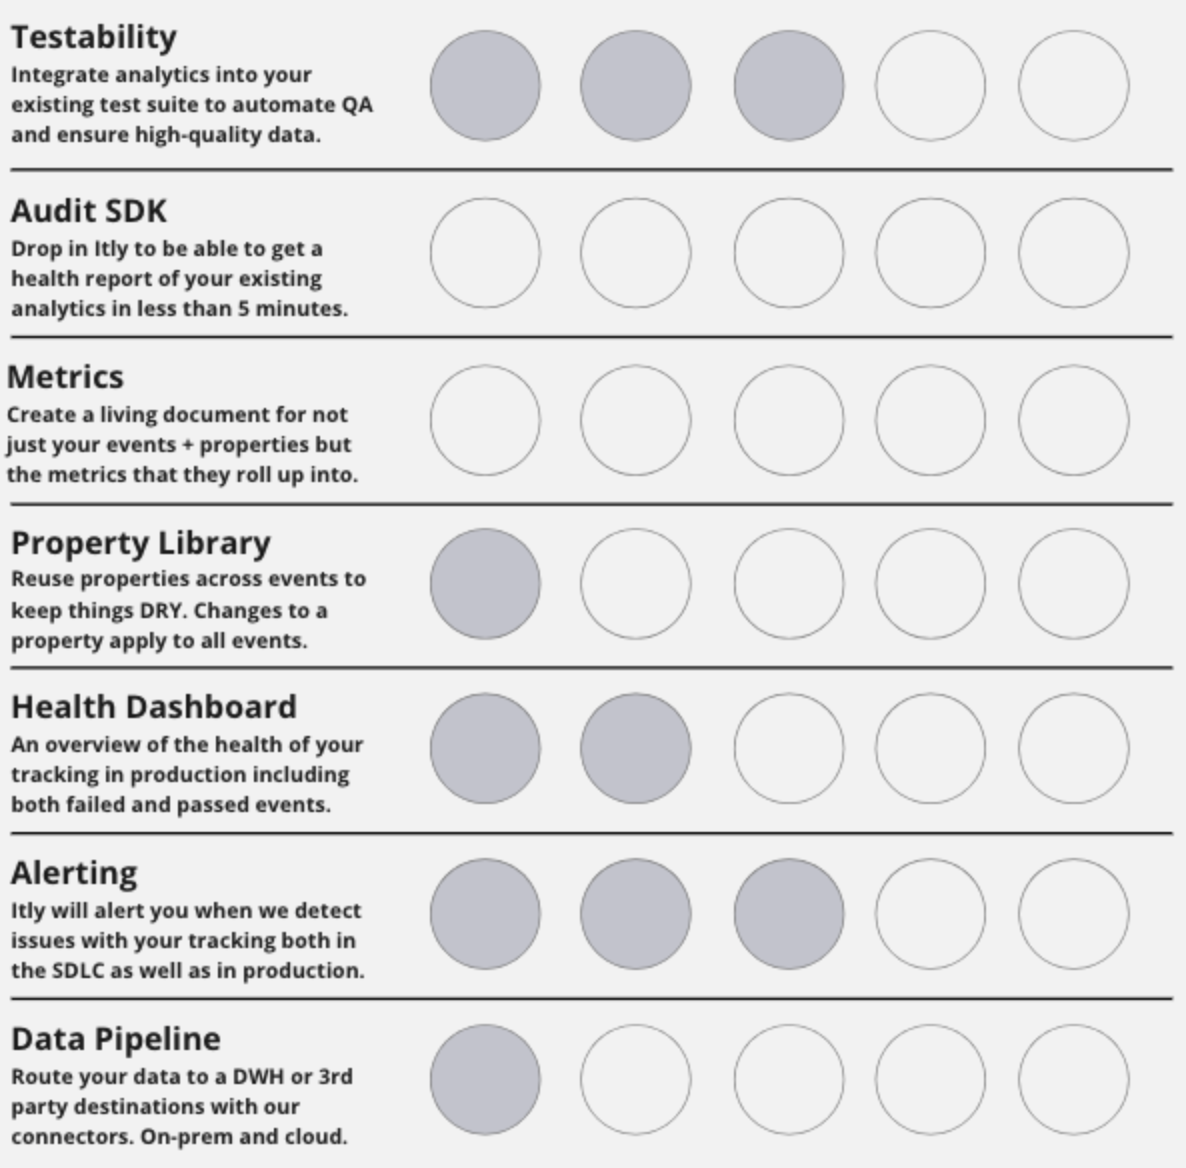
\includegraphics[width=\textwidth]{images/iteratively/dot-voting-example.png}
  \captionof*{figure}{Dot-voting example}
  \label{fig:iteratively-dot-voting-example}
\end{minipage}
    \caption{Iteratively: Product/Market fit}
    \label{fig:iteratively-product-market-fit}
\end{figure}

\myindex{Iteratively} had developed a combination of an online design tool that created a schema for third-party in-app analytics tools. They also provided build tools and a small client-side SDK (\emph{i.e.} a mobile \Gls{sdk}) which validated the schema had been implemented adequately in the mobile app. %, where all the data from the schema and only the data from the schema would be collected by the relevant mobile analytics SDK.
Iteratively's SDK was intended to limit the collection to only the data contained in the schema. This was intended to stop the collection of other data (such as \Gls{pii} data). Through the use of the SDK, the build tools, and the online design tool development teams and their colleagues with other roles such as marketing, product, and so on could have a consistent and coherent understanding of the data that was being collected. Of interest to this research, they did not address the collection of errors or failures such as crashes in their SDK.

\myindex{LocalHalo} are a good example of a small development team who chose to include several mobile analytics SDKs into their mobile app where each SDK (and the respective service) was chosen to provide orthogonal data. They chose \href{https://sentry.io/}{Sentry} for technology facing analytics and \href{https://mixpanel.com/}{mixpanel} for product (business facing) analytics. Although Sentry provides APIs~\footnote{\url{https://docs.sentry.io/api/}} for integration and data forwarding~\footnote{\url{https://docs.sentry.io/product/data-management-settings/data-forwarding/}} and mixpanel provides data pipelines~\sidenote{\url{https://mixpanel.com/data-integrations/}} LocalHalo did not use these. In contrast for the large commercial project data integration was deemed vital by the organisation in order to facilitate ongoing and \emph{ad-hoc} analysis across multiple sources of information. 

In the case of the corporate project, \myindex{C1}, the product (the mobile analytics tool) also had to fit at the level of the engineering organisation where the mobile analytics needed to be ingested into the corporation's `data-lake'. 

Finally for this topic, despite many mobile analytics SDKs, there may be situations where none provides the answers the developers seek. As a concrete example, \myindex{SmartNavi} uses \myindex{Firebase} and \myindex{Google Analytics}, mainly for tracking the popularity and the use of the app's features. The app also incorporated Fabric Crashlytics for crash reporting. Nonetheless the developer explained none of these analytics products provided analytics related to software running in the background, as a background process on Android. SmartNavi provides GPS services to other apps and runs in the background. As the Android Platform has evolved Google has embedded restrictions that limit and constrain background processes which meant the SmartNavi software is suspended (paused) by Android. The developer would like to improve the app's behaviours when it runs in the background but lacks the analytics to do so.

\subsection{Actionable Reports}
\textbf{Actionable Reports} are reports the developers can use to decide on what should be done to address concerns presented in the reports. % c.f. actionable metrics https://effectivesoftwaredesign.com/2021/03/23/lean-startup-principles-vanity-metrics-and-actionable-metrics/

Several of the app-centric case studies materialised because the respective development teams became aware of excessive and chronic error rates for their mobile apps. % Kiwix, Catrobat, C1
These projects (\myindex{Kiwix}, \myindex{Catrobat} and \myindex{C1}) had not managed to materially reduce the high crash rates directly and they were happy to receive help and insight in how to apply the information from the reports in their work. At the time they lacked the wherewithal to do so unaided. With interventions, including those that were part of this research, each of the development teams were able to materially improve the error rates of their respective apps.

None of the currently available mobile analytics tools seen during this research were able to pinpoint the causes of failures, instead they identify one or more effects \emph{e.g.} the app crashes, or is stopped by Android because it became unresponsive. The action-ability comes in part from the meta-data collected by the various mobile analytics tools which helped in bug localisation and in part from the characteristics and patterns contained in the reports. The Moonpig developers, for example, were sometimes able to identify a highly likely reason for the failure from the contents in the reports. They took action by modifying the application's source code.

\myindex{Android Vitals} aims to highlight emerging problems with a deployed app. For instance if there is an acute and significant increase in the crash rate for the production release(s). It also provides cross-connections between problems found in Google Play's pre-launch reports and failures that occur in production. Developers found some of the reported failures easy to comprehend and address, others have been much less tractable. Several of the developers who use Crashlytics said they preferred using it over Android Vitals for comprehending crashes. \myindex{Crashlytics} provided more information than Android Vitals and the reports were easier to digest therefore the Crashlytics reports were more actionable than those from Android Vitals.

As discussed in the flaws topic (\secref{section-flaws-in-the-analytics}, \secref{section-flaws}) various reports have flaws, for instance in their aggregation. There is scope to improve the mobile analytics tools through improving the matching process in the data aggregation (for instance, where there are fragmented `failure clusters') and in the analysis across multiple legitimate failure clusters (such as across all \texttt{NullPointerExceptions}) to help identify underlying flaws in the development of the app.

The \myindex{Moonpig} case study provides an illustrative example of how the development team was able to take proportionate and measured action as the crash-rate of their Android app increased. The cause was related to a known and documented issue with a third-party software library, RoboSpice. There was a clear correlation where the crash-rate increased on newer Android releases. The team was able to evaluate and estimate an appropriate timescale to replace that library by revising the application's source code. They were able to schedule the release to suit other strategic objectives rather than rushing to push out a `fix' of the app.

The release management reports in Google Play Console (that incorporate various Android Vitals reports pertinent to the latest release for the 7 days post release) were highly actionable for the Commercial project. The development team were able to abort releases that had unexpected increases in failure rates before those flawed releases adversely affected swathes of the userbase.

\subsection{Integration into workflows}~\label{tata-integration-into-workflows-topic}
Integration into workflows is the ability of a given mobile analytics tool/service to be integrated into development team's workflows. These workflows include bug tracking and release management. Some mobile analytics tools provide facilities where developers can mark and/or annotate elements in the reports, for instance to remove a crash cluster from the main report or to provide a bug-tracking link to help the developers streamline their work when using mobile analytics.

When cross-references are stored in mobile analytics, viewers can see which of the issues have been reported (and by inference which have not been acknowledged e.g. because the issues are new to the team).

\begin{figure*}
    \centering
    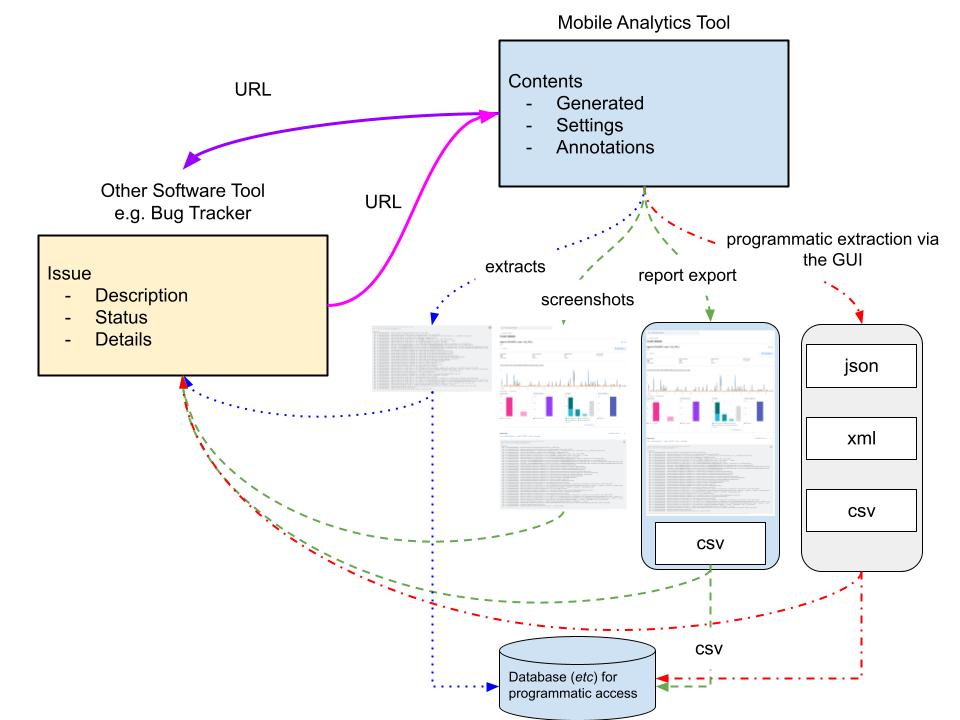
\includegraphics[width=\linewidth]{images/rough-sketches/integration-of-mobile-analytics-tool.jpeg}
    \caption[Addressing the contents of Mobile Analytics reports]{Addressing the contents of Mobile Analytics reports\\Source: Google Drawing \href{https://docs.google.com/drawings/d/1y7QP8UK7ugl0DzWIeH4udRxwsVMHjyQ6Am0qW6glkdE/edit?usp=sharing}{online here}.}
    \label{fig:addressing-the-contents-of-mobile-analytics}
\end{figure*}

Figure \ref{fig:addressing-the-contents-of-mobile-analytics} illustrates various aspects of integration between mobile analytics and other software tools such as bug trackers. The mobile analytics tool provides reports in a graphical user interface. On the web, the report has a URL (it may not be directly addressable in a mobile app equivalent tool) and visiting the URL with a suitably authenticated account results in the report being rendered if the mobile analytics service is working adequately. The mobile analytics tool \emph{may} provide interactive elements in the report page, for instance to hide the issue, to annotate the report, to modify the selection criteria. 

Some tool's URLs include structural elements for instance to vary the dates or the duration of the report (24 hours, 7 days, \emph{etc.}). And some tools provide for easy export of elements of the report or of the entire presentation of the report \emph{e.g.} as a PDF file or an image file. Another approach, albeit one seldom supported officially is to write code to extract content programmatically; we did so as part of this research and developed vitals-scraper to extract content from Android Vitals.

\newthought{Why do these aspects matter? } 
Development teams often want to identify and track bugs including any code changes made with the aim of fixing the bug. Mobile analytics may be the source for the information about the bug and when the issue in the bug database includes pertinent information from the mobile analytics tool the development team can use that information to help understand the bug. \emph{The ability to cross-link the mobile analytics report and the issue in the bug tracker can enable team members to review the current, live information in the peer system.} 

Figure \ref{fig:addressing-the-contents-of-mobile-analytics} includes five distinct mechanisms to integrate individual reports, or at least some of their contents.
\begin{enumerate}
    \itemsep0em
    \item The web address or URL: for some reports the URL may include structural elements that affect the contents of the report.
    \item Exports of the report: these are generally as a PDF or as a \Gls{csv} file (which would include a subset of the entire report).
    \item Ubiquitous screenshots: some web browsers \emph{e.g.} Google Chrome limit the screenshot to the viewport (what's visible in the web browser), others \emph{e.g.} Firefox provide options to take a screenshot of the entire report.
    \item Content extracts: \emph{e.g.} using copy+paste links on screen, \emph{e.g.} Android Vitals does so for the stack trace of crashes and for the thread dump of ANRs.
    \item Programmatic extraction via the GUI: commonly known as screenscraping\sidenote{Note: some mobile analytics tools may provide API access to obtain the reports and/or the contents of the reports however none was discovered during the case studies.}. 
\end{enumerate}

Text-based content can be stored and processed relatively easily (analysis and processing of graphically-based PDF reports and images is beyond the scope of this research). 

\newthought{Report exports: }
Android Vitals provides various exports as files of comma-separated values (\Gls{csv} files).  However, these are encoded in a UTF-16 character encoding, an encoding used by less than 0.005\% of websites according to~\sidecite{w3techs_utf16}, via~\sidecite{wikipedia_utf16}. UTF-16 content proved awkward to parse programmatically which complicates and adds friction to any analysis or integration of these CSV reports from Android Vitals.

\newthought{What content does a URL point to? }
Where the URL points to can affect the integration where a) the underlying content has been updated and the reference was intended to be of a snapshot in time when an issue occurred, b) the underlying content \emph{has not} been updated yet the url indicates the view should be relative to the current time and date, or c) where the content is no longer available, at all.

The URLs may point to persistent historical reports or to recent, periodically updated, reports. Some reports are also updated as new releases of an app go into production. The URLs and/or the contents often have a finite life. Trend analysis might be available within the mobile analytics tool, otherwise it can be performed using snapshots of reports for a range/set of consistent periods \emph{e.g.} snapshots taken on the first day of every week can be used to perform trend analysis. Retention policies applied by the mobile analytics service may mean the underlying data is deleted; for example Firebase Crashlytics only retains crash stack traces, \emph{etc.} for 90 days~\sidecite{firebasesupport2022_crashlytics_data_retention_policy}. The data is then deleted from Firebase Crashlytics. Therefore, development teams would need to preserve the contents of the reports if they wish to perform longer-term analysis or for auditing, \emph{etc.}


\newthought{Integration of event and content verification: }
As mentioned earlier in this chapter, \hyperlink{tata-design-of-mobile-analytics-events-and-content}{Iteratively's various software tools}  helped the teams design and implement the desired mobile analytics correctly in a mobile app. Their tools were primarily involved before the app was tested or released, nonetheless they included a short duration view of the mobile analytics events being emitted by the app when the app was being used.

In comparison, the release management section of Google Play Console is integrated into the rest of the services and reports offered in Google Play Console. Therefore it \emph{knows} the details of each release and is able to perform calculations and analysis accordingly for every new release of an app. In the commercial project the product owners were also able to use the release management reports to help them work with the developers to make decisions on staged rollouts including, when necessary, stopping the rollout entirely. The release management tools were a core part of release management and rollout for the overall team. % C1: Release management functionality including reports, alerts, history, and so on can enable developers to understand what's happening in terms of the adoption and use of their app releases. 

The final topic for the integration into workflows is on pipeline integration between mobile analytics tools/services and other high-volume data processing systems used particularly in larger tech-savvy enterprises. In the corporate app-centric case study the organisation required the product's development team to integrate any and all of the mobile analytics services where such integration was available. These were paid-for integrations where the service provider charges for the integration and for the data processing aspects. The app developers did not necessarily use the internal data lake often, instead the Operations and Site Reliability teams did, therefore the details are beyond the scope of this research.

\subsection{API access to analytics outputs}
None of the mobile analytics tools encountered during the research provided complete access to the outputs using APIs. Furthermore, the ability to record and preserve copies of visual reports (as well as the underlying data) facilitates both practical use of the data in the field (for instance to record the information in an issues tracking database) and for further analysis and research. 

API access to mobile analytics has been requested previously for Google Play's Developer Console~\sidecite{stackoverflow2013_getting_statistics_from_google_play_developer_console_with_an_api} and various people have developed code that interfaces with Google Play Console in an attempt to provide automated, scripted access to the content.

\begin{kaobox}[frametitle=Opensource projects to download data from Google Play Console]
Two examples of opensource projects that were created to download data include:

googleplay\_dev\_scraper~\sidenote{  \href{https://github.com/tmurakam/googleplay_dev_scraper}{github.com/tmurakam/googleplay\_dev\_scraper}}, provided mechanisms to automate the downloading of the \Gls{csv} monthly reports rather than the live reports. It was last updated in 2013 so no longer current. 

There was also the Andlytics opensource app that provided developers with access to data from their Google Play Console account~\sidenote{\href{https://github.com/AndlyticsProject/andlytics}{github.com/AndlyticsProject/andlytics}}. 
However this project also ceased active development for various reasons, probably because Google chose to restrict access to the underlying data in 2019~\sidenote{\href{https://github.com/AndlyticsProject/andlytics/issues/766}{\nolinkurl{github.com/AndlyticsProject/andlytics/issues/766}}}. % See also the historic posts by the project on Facebook for screenshots and updates https://www.facebook.com/Andlytics/
\end{kaobox}

\newthought{Using Web-scraping for ad-hoc integration: }
Web-scraping of content from web-sites continues to be a frequent activity performed by many people and services. Web-scraping is used in many fields including bioinfomatics, where the authors discussed why web-scraping was still necessary in a world full of API's~\sidecite{glez2014_web_scraping_in_an_API_world}. A more recent paper by~\sidecite{diouf2019_web_scraping_state_of_the_art_and_areas_of_application} briefly presents various inefficiencies in web scraping. Curiously this paper singles out journalism as an under-served area despite it being written about 7 years earlier in Chapter 4 of~\sidecite{gray2012_the_data_journalism_handbook} (and also covered in a more recent version of the book,~\sidecite[][pp. 133, 238]{bounegru2021_the_data_journalism_handbook}. Suffice to say, web-scraping is a topic that has been written about, albeit not in the context of scraping content from mobile analytics web interfaces. 

We developed \myindex{Vitals Scraper} as an opensource project~\sidecite{vitals_scraper_github_package} and released it as an \acrshort{npm} package~\sidecite{vitals_scraper_npm_package} to address the issue of the lack of access to the outputs of Google Play Console and Android Vitals. Doing so demonstrated the necessity, viability, and some of the maintenance challenges of writing automated software for web-scraping of outputs from Google Play Console with \myindex{Android Vitals}. 

Enterprise-grade mobile analytics services provide mechanisms to export data to homogeneous data storage platforms~\sidecite{androiddevelopers2015_integrate_play_data_into_your_workflow_with_data_exports}; for instance Google Analytics tools export content to Google Cloud Storage~\sidenote{\href{https://support.google.com/googleplay/android-developer/answer/6135870?hl=en-GB}{support.google.com/googleplay/android-developer/answer/6135870}}, and to automate the process~\sidenote{\href{https://cloud.google.com/bigquery-transfer/docs/play-transfer}{cloud.google.com/bigquery-transfer/docs/play-transfer}}. Microsoft App Center is unusually complete and provides a comprehensive set of open APIs \href{https://openapi.appcenter.ms/}{openapi.appcenter.ms/} as well as the ability to export analytics data to Azure \href{https://docs.microsoft.com/en-us/appcenter/analytics/export}{docs.microsoft.com/en-us/appcenter/analytics/export} and even export data for individual users \href{https://docs.microsoft.com/en-us/appcenter/gdpr/analytics-export}{docs.microsoft.com/en-us/appcenter/gdpr/analytics-export}. Google Analytics provides various reporting APIs including those for Exceptions~\sidenote{\href{https://ga-dev-tools.web.app/dimensions-metrics-explorer/exceptions}{ga-dev-tools.web.app/dimensions-metrics-explorer/exceptions}} which are collected by Firebase Analytics for both Android and iOS apps~\sidenote{\href{https://developers.google.com/analytics/devguides/collection/firebase/android}{\nolinkurl{developers.google.com/analytics/devguides/collection/firebase/android}}}. % See also their github site that underpins the docs https://github.com/googleanalytics/ga-dev-tools

Some of the mobile analytics providers offer developers customisation options such as custom dashboards and reports in Sentry \href{https://docs.sentry.io/product/discover-queries/uncover-trends/}{\nolinkurl{docs.sentry.io/product/discover-queries/uncover-trends}}.

As a broader observation, various companies provide app analytics services where they obtain the underlying data % See the discussion for https://stackoverflow.com/a/49893656/340175
and aim to provide easy to use, attractive, and actionable reports; examples include \href{https://appfigures.com/}{appfigures.com} and \href{https://www.data.ai/en/}{www.data.ai/en} (previously known as AppAnnie). Appfigures also publishes status reports for the performance of Google Play and Apple's App Store Connect service, these track the publishing performance of these two app stores; at the end of February 2022 they observed Google has been several days late publishing their free daily reports. % Screenshots have been recorded for posterity and are available in my research's appfigures.com folder. 


\subsection{Android Vitals}~\label{tata-android-vitals-topic}
As Android Vitals features in every one of the app-centric case studies it has been possible to consider it in greater depth than the other mobile analytics tools investigated in this research. For example, having access to Android Vitals enabled comparisons across case studies and across multiple apps in and across those case studies. Having access also led to direct investigations of the Android Vitals on all the app-centric case studies. Flaws could be compared, for instance: 1) where the second country in the userbase graph was mistakenly used for the title of that report, 2) where a userbase appears to be negative when more users were lost and gained over the lifetime of the app, as shown in Figure \ref{fig:PocketCode-Lifetime-User-KPIs-2020-jan-24}. This has been observed for several of the apps in the case studies, a pattern for when this occurs has yet to be determined.

\begin{figure}
    \centering
    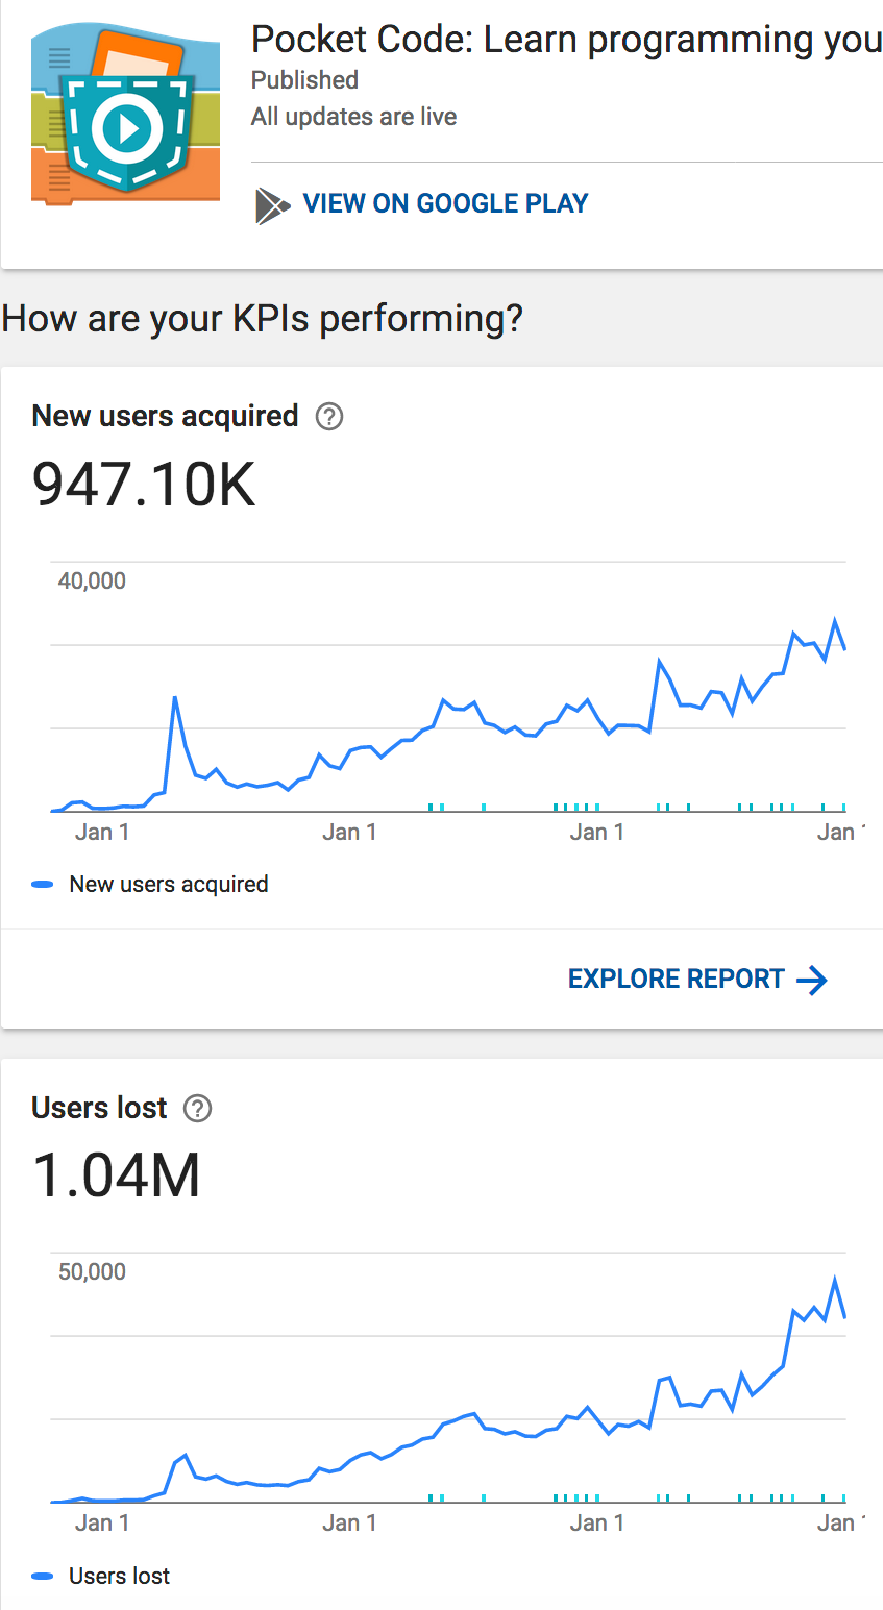
\includegraphics[width=0.75\linewidth]{images/android-vitals-screenshots/catrobat/PocketCode-Lifetime-User-KPIs-2020-jan-24b.pdf}
    \caption{Google Play Console Dashboard for PocketCode Lifetime User KPIs on \nth{24} Jan 2020}
    \label{fig:PocketCode-Lifetime-User-KPIs-2020-jan-24}
\end{figure}


\subsubsection{Which apps can Android Vitals help?}~\label{tata-which-apps-can-google-vitals-help}
As Google only provides various reports in Android Vitals once they decide enough data exists to preserve the privacy of end users Android Vitals provides little for developers of less popular apps. 

Based on very rough approximations combining my case studies with AppBrain's download statistics to \nth{19} June 2019, shown in figure \ref{fig:appbrain_download_statistics_jun_2019}\cite{appbrain_download_statistics_june_2019}, of the total populations of app developers:
\begin{itemize}
    \item 3\% to 4\% (those with 100,000 to 500,000 total downloads) will get limited value as at least one report will be provided.
    \item < 1\% (those with 500,000 to 1,000,000 total downloads) will get some value as many of the reports will be provided, but not all.
    \item 1\% (those with > 1,000,000 total downloads) will get extensive value as most/all the reports will be provided.
\end{itemize}

\begin{figure}[!htbp]
    \centering
    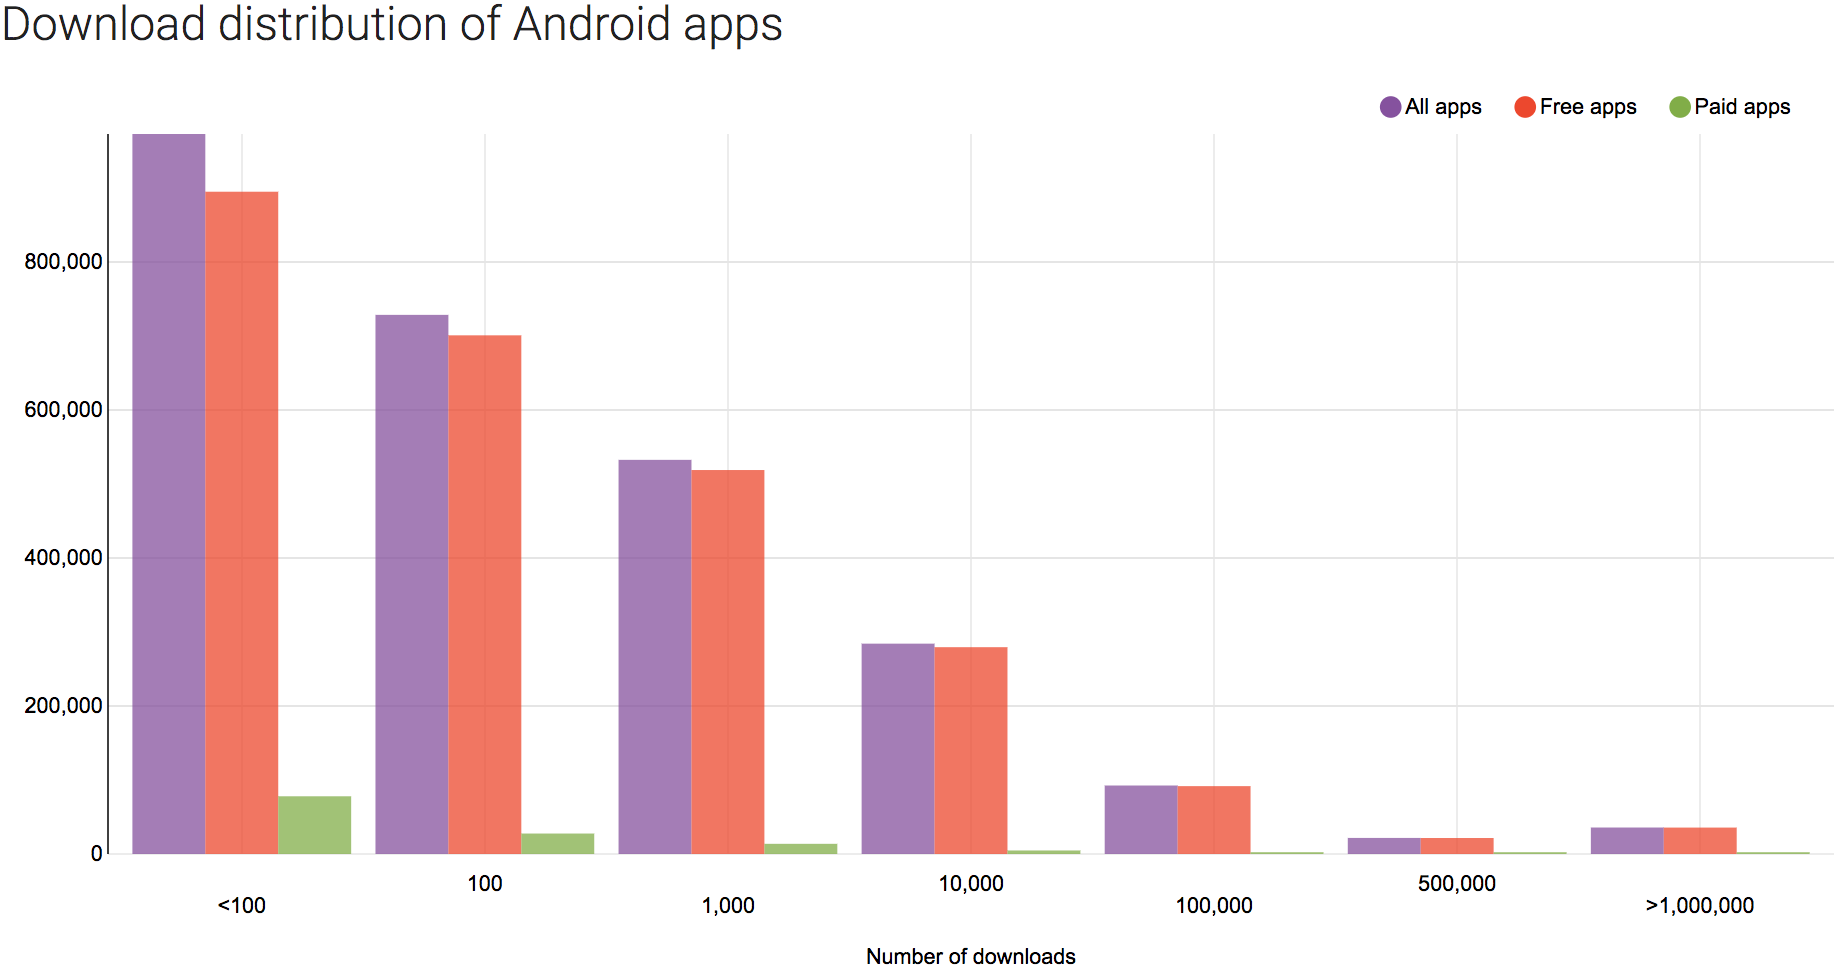
\includegraphics[width=\textwidth, keepaspectratio]{images/appbrain/AppBrain_Download_Statistics_20-Jun-2019.png}
    \caption{AppBrain: Download distribution of Android apps (June 2019)}
    \label{fig:appbrain_download_statistics_jun_2019}
\end{figure}

\subsubsection{Limitations in using Android Vitals for Observability}
Observability provides two key benefits according to~\sidecite{lightstephq2021_observability_will_never_replace_monitoring}: 1) monitor key signals, and 2) understand changes in a system. Mobile analytics facilitates observability of mobile apps, and in particular Android Vitals facilitates the observation of app startup times, performance, ANRs and crashes that occur when an app starts-up. However the inability of storing and analysing the data over time in Android Vitals (beyond the standard reports and recent failure details) limits the ability to observe and analyse stats and/or failures over time.

\subsubsection{Who gets sufficient usage to see more detailed reports?}~\label{tata-sufficient-usage-to-see-more-detailed-reports-topic}
Our limited insight into Android Vitals already indicates that reports are only provided when there is sufficient data collected to 'prime the pump'. It may be possible to estimate how many apps of those in Google Play Store are likely to have enough volumes of usage data. Google makes various recommendations for developers on how to apply the results Android Vitals reports \href{https://developer.android.com/distribute/best-practices/develop/android-vitals}{\nolinkurl{developer.android.com/distribute/best-practices/develop/android-vitals}} however the developers can't do much until Android Vitals actually shows them the data. For apps with less than about 50k active installs \emph{("Installs on Active Devices (devices online in the past 30 days with this app installed)}." according to Google Play Console's tool tip). These counts are around 20\% to 30\% of the total install count for various apps used in our research \emph{e.g.} the active installs would be around 20k for an app that shows at having 100,000+ [total] installs to end users in Google Play.

Data provided by AppBrain~\cite{appbrain_download_statistics_june_2019} was used to estimate the populations of apps that are not likely to generate enough data to see various reports in Android Vitals.
% wikimedes 5373 active installs - Crash rate by app version only (not device or Android version).
% wikimedzh 3769 active installs - no Android Vitals reports
% wikimedfa 2807 active installs - no Android Vitals reports
% 
Based on Android Vitals reports for Kiwix custom apps we infer that few apps with less than 20,000 total installs will have any detailed reports; WikiMed in Spanish has 5,373 active installs and has one report, for crash rate by app version. None of the other reports are available for this app. The threshold for when there is enough data for Google to provide a report depends on various factors, so the total installs is a proxy measurement and imperfect. Therefore Android Vitals is unlikely to offer much value for developers of (973,381 + 730,419 + 553,261 + 284,634) apps i.e. 2,541,695 apps in Google Play. For the next 92,678 the value of Android Vitals might increase somewhat, depending on how their app behaves and their user-base (e.g. are they on a few Android versions or spread across a spectrum - the larger the spread the less likely the reports will have data). And so on. By my admittedly limited view into the overall data set, Android Vitals is best placed to help the developers of the top (21,728 + 35,854) 57,582 apps, approximately 2\% to 3\% of the total population (2,691,955 apps). These apps (according to AppBrain's data on library use) are also more likely to use Firebase, Crashlytics, etc. so also have some of the run-time data available from these sources in addition to Android Vitals.

My work is to investigate two broad sources of data - data collected by the operating system (here effectively what appears in Android Vitals) and data collected using in-app libraries, particularly mobile analytics, it could include heatmapping (\emph{e.g.} Appsee, found in over 790 Android apps with over 375 million downloads~\sidecite{appbrain_appsee}), crash handlers, etc. to provide feedback to measure how well the development team did in terms of testing and code quality. What they learn could also be useful to help them improve how they develop and test their apps in future, particularly with the greater detail mobile analytics (particularly Firebase) can provide the team.

\subsubsection{False positives}~\label{tata-false-positives-topic}
Not all issues flagged by \myindex{Android Vitals} are valid problems that need to be acted on for a given app. For example, in the Kiwix app-centric case study, Android Vitals sometimes reports excessive network usage running in the background while the device is running on battery, as shown in figure \ref{fig:android_vitals_excessive_network_usage}. As the Kiwix app is designed to enable users to download sometimes extremely large files, and to do so in the background, this warning is to be expected and not a bug - it's a feature. App developers could choose to modify their app's behaviour to increase their score in Android Vitals; the effects could actually improve the app's behaviour for end users, or potentially in a similar fashion as some vehicle manufacturers who implemented `anti-defeat' devices to improve the measured results of their vehicles during authorised testing~\sidecite{canis2016_volkswagen_defeat_devices_and_the_clean_air_act_faqs, schuelke_leech2018_ethical_dilemmas_for_engineers_in_the_development_of_autonomous_systems}.

% Isabel mentions why devs don't use paper: https://scholar.google.com/scholar?hl=en&as_sdt=0%2C5&q=emerson+murphy+hill+static+analysis&btnG=

\begin{figure}[!htbp]
    \centering
    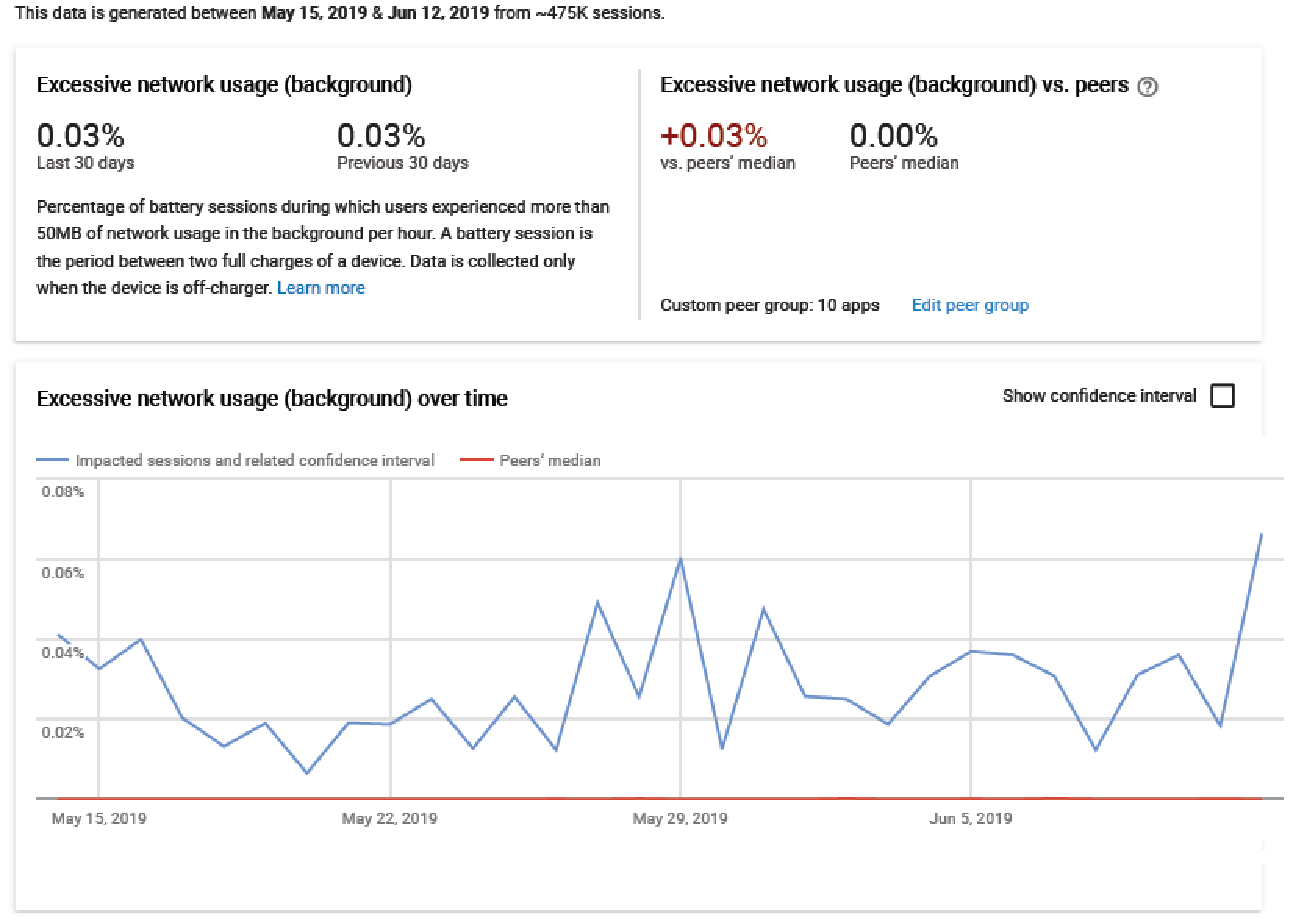
\includegraphics[width=\textwidth, keepaspectratio]{images/android-vitals-screenshots/kiwix/Excessive_network_usage_by_kiwix_15_jun_2019.pdf}
    \caption{Excessive background network usage on battery}
    \label{fig:android_vitals_excessive_network_usage}
\end{figure}



\section{Utility}~\label{tata-utility-section}
Utility addresses practical and pragmatic aspects of developers using mobile analytics to achieve their purposes. It's a close cousin to \secref{section-fit-for-purpose} and considers three discrete lower-level themes: efficacy of the mobile analytics tool(s), the benefits of combining tools, and bug-localisation.

An orthogonal topic is included in this section as Google has provided various online tools to help developers pre-release of their Android apps. One in particular, pre-launch reports, compares failures found pre- and post- release and is instructive in how well automated platform-provided checks and tests might help developers reduce the incidence and/or severity of post-release failures.

\subsection{Efficacy of the tool}
% 4 findings currently: Android Vitals, Kiwix, Moodspace (email/empirical studies), Moonpig (email/empirical studies).
Efficacy of tools considers how efficient and how effective is the tool, i.e. how efficacious is the tool? Did it achieve the objectives it claims to achieve?\todo{These don't quite align with the rest of this topic and should do. TODO - align them :)}

\newthought{Android Vitals: } 
The current design of \myindex{Android Vitals} includes notifications and alerts, the use of colour, comparisons, and so on are all intended to get the attention of the developers and help the developers focus on egregious issues. During the app-centric case studies several project teams provided examples of where these worked. Comparisons with peer apps helped inform and motivate the project team for the commercial app, \myindex{C1}, albeit the product owners appeared to be more interested than the core development team. (Note: the comparison is provided per developer account, per app, rather than per logged-in user, in Google Play Console, \emph{i.e.} anyone able to login to see the app's analytics will see the same set of peer apps.). 

\begin{quote}
    ``\emph{Seeing your app in comparison to apps of peers provides some great motivation to step up your game.}'', Moodspace (2019).
\end{quote}

\begin{quote}
    ``\emph{...we noticed them by monitoring with Crashlytics/Firebase, I think specifically in the last case we got a crash velocity alert}'', Moonpig (2020).
\end{quote}

For the Kiwix project, the project leads were convinced by the reports provided in \myindex{Android Vitals} that an interim bug-fix release would be worth the effort of making and releasing quickly in order to materially reduce the crash rate for the core app (it was - as measured by Android Vitals).

\newthought{\myindex{Crashlytics} and \myindex{Microsoft App Center}: }
both include in-app crash reporting that project teams preferred using over the equivalent reports in Android Vitals. The reports were more actionable for at least two main reasons, one systemic and the other because of how Google currently processes and reports on crashes in Android Vitals. 

The systemic reason is that in-app \Gls{sdk}s often offer facilities that enable developers to get the apps to report information in addition to crashes. The information may include: \gls{glossary-breadcrumbs}, custom data, handled exceptions (non-fatal errors), and so on. As Android Vitals relies on data that is logged when an app is terminated it does not have access to any of these additional (and optional) data.

Android Vitals limits what it reports to the app developers. Here are two key examples.

\begin{enumerate}
    \item Android Vitals currently doesn't present the optional \texttt{message} parameter \emph{e.g.} the parameter `\texttt{s}' in Java's \texttt{NullPointerException(String s)}~\footnote{In full, \texttt{NullPointerException(String s)
Constructs a NullPointerException with the specified detail message.} Source:  \href{https://docs.oracle.com/javase/7/docs/api/java/lang/NullPointerException.html}{docs.oracle.com/javase/7/docs/api/java/lang/NullPointerException.html}}. While some crashes can be determined without this message (and indeed some fatal exceptions don't include a message as it's an optional parameter) others have only been determined by the developers when the developers have seen the contents of the messages.
    \item Android Vitals also only provides reports once internal thresholds have been reached whereas the in-app analytics tools report even isolated events. With Android Vitals Google has chosen to protect user's privacy (possibly relatively rather than absolutely) compared to their other mobile analytics product offerings such as Firebase Analytics and Firebase Crashlytics.
\end{enumerate}

This second example was raised as a requested improvement during the interview with Ian Alexander of Moodspace:
\begin{quote}
    ``\emph{The only issue I have with core vitals is that I can't see them all! We are by no means a big app, so don't have enough data to meet Google's standard for anonymised results, so results for most of the core vitals are hidden. I don't quite understand why this should be the case as the headline figure of your apps performance surely doesn't have to rely on anonymous data? Whereas the drilled down details of a core vital should be anonymous, so maybe the details view could just be blocked instead of hiding the entire core vital? To provide context, \myindex{MoodSpace} had at least 4k monthly users, so there must be plenty of apps which get little or no use form core vitals, simply from them being hidden.}'' Moodspace (2019).
\end{quote}

Auto-instrumentation, for example, provided by Sentry and as seen in the \myindex{LocalHalo} project, can also help developers to identify contributory factors to failures. In the \myindex{LocalHalo} case study, \myindex{Sentry} clearly identified the servers were no longer functional. This occurred months after the project and the app were no longer supported, were the project actively maintained there was sufficient information in the analytics to help the development team focus their attention on the servers. In the commercial project their mobile analytics services did not include equivalent auto-instrumentation, instead one of the developers wrote similar code to log (\emph{i.e.} record) web server responses. In doing so they inadvertently caused the newly released version of the Android app to crash frequently. Here what is noteworthy is that developers sometimes have to write their own code to augment the functionality provided by a mobile analytics service. It's pertinent to mention that auto-instrumentation can also have flaws that include causing the app to crash. A similar example, albeit for a different third-party SDK was when \myindex{Facebook}'s SDK led to high app crash rates.

\subsection{Benefits of combining tools}
% 6 findings currently: 2 - Kiwix, 3 - LocalHalo, 1 - Moonpig:
% Benefits of combining mobile analytics tools: an observation of benefits developers can obtain through combining their use of several mobile analytics tools.
    
\myindex{Moonpig}'s development team actively combined \myindex{Firebase Crashlytics} and \myindex{Google Analytics} for diagnostics in addition to the information available in Android Vitals. They estimated they used \myindex{Android Vitals} approximately 30\% of their time to identify flaws and issues related to their Android app.
%
They also incorporated in-app analytics by using \myindex{Firebase Analytics} which recorded analytics related to how the users use the mobile apps and whether errors or other problems occurred while the app was being used. 

Some crashes were only reported in \myindex{Android Vitals}, \myindex{Moonpig}'s hypothesis was that as \myindex{Crashlytics} waits to send crash reports until the app next restarts, some users never restarted the app therefore those crashes remained unreported \emph{even if crashlytics had detected and recorded them}.

subsection{Bug-localisation}
% 4 - Moonpig, 1 - Kiwix, 1 - SmartNavi (discussion): 
% Bug-localisation: features in a mobile analytics tool that may enable developers to localise one or more bugs.

\myindex{Moonpig} provided several examples of how mobile analytics helped with bug localisation. The most instructive example is where there was a clear correlation between an increase in the crash rate of the app and newer Android releases. The development team:

\begin{enumerate}[label=(\alph*)]
    \item understood the correlation, in part as the early effects were documented by the developer of the relevant third-party software library: \myindex{RoboSpice}, and 
    \item they were able to make suitable purposeful, controlled improvements to the app where they were able to revise the codebase so the app could be improved despite the removal of RoboSpice.
\end{enumerate}

With Kiwix, Android Vitals provided sufficient information to help the developers to gauge the probable impact of various flaws that emerged in use of the family of Android apps. The reports weren't necessarily comprehensive or complete so they didn't necessarily pinpoint something the developers could address. Similarly for the \myindex{SmartNavi} Android app the developer was able to determine the crashes \emph{that wouldn't be fixed} because the analytics reports indicated the failures were a) sufficiently sporadic and infrequent, and b) on devices that weren't available outside their respective region \emph{e.g.} China. So the reports helped the developer of SmartNavi to make appropriate triage decisions - the action was to take no further action! 

\subsection{Pre-launch reports}~\label{tata-pre-launch-reports-topic}
Pre-launch reports are an intrinsic part of Google Play Console and the pre-launch~\sidenote{Google provides a current overview of pre-launch reports online \href{https://play.google.com/console/about/pre-launchreports/}{\nolinkurl{ play.google.com/console/about/pre-launchreports}}.} report includes automated testing of pre-release apps. These reports are generated by a combination of static analysis tools and automated `testing' performed by a software test facility called Robo, which is also used in the Firebase Test Lab service.

Pertinently, \myindex{Google Play Console} identifies issues that are found in both the pre-launch testing and in production, an example is provided in \secref{aiu-pre-launch-reports}. They also automatically select the top five languages~\footnote{More probably they actually select the locales which are more specific than simply a language.} based on the app's userbase~\sidecite{play_console_use_a_pre_launch_report_to_identify_issues_2022}, which is a simple example of how mobile analytics can be used to drive software testing.

\begin{quote}
``\emph{If you use pre-launch reports to identify issues with your apps, crashes found during testing are listed with your app’s crashes and \Gls{anr}s. However, because crashes found while generating a pre-launch report come from test devices, they don’t affect your crash statistics.}''~\sidecite{play_console_help_view_crashes_2019, play_console_help_understanding_pre_launch_reports_2022}.    
\end{quote}

As the \myindex{GTAF} project noted, the crashes reported in pre-launch reports do not necessarily affect end users. Conversely the pre-launch report automated testing does not find all the failures that affect end users. (Dua \& Zikr app).


Unfortunately the pre-launch reports started reporting false positives claiming that apps were crashing during the automated testing; and this was exacerbated by the tardy responses by the Google engineering team and inadequate `fixes' that didn't work~\sidecite{google2020_pre-launch-reports-false-positives}. % And see also https://github.com/firebase/firebase-android-sdk/issues/2161 https://stackoverflow.com/questions/64706041/fatal-exception-firebase-messaging-intent-handle-java-lang-noclassdeffounder https://forum.unity.com/threads/error-during-google-app-submission-java-lang-noclassdeffounderror-aewt.1005593/
Some app developers chose to bypass the pre-launch reports so they could release new versions of their apps. These false positives adversely affected several of the app-centric case studies including the commercial project who had experienced other flaws in the pre-release release tracks serving outdated releases to key stakeholders. The pre-launch report for the WikiMed app in Arabic also reported this issue, see Listing \ref{listing:kiwix-wikimed-ar-pre-launch-report-crash}. The crash appears to be in the unrelated YouTube app installed on that device. 

\begin{listing}
\begin{minted}[fontsize=\tiny,obeytabs=true,tabsize=2]{java}
FATAL EXCEPTION: Firebase-Messaging-Intent-Handle
Process: com.google.android.youtube, PID: 27568
java.lang.NoClassDefFoundError: aewt
\end{minted}
\caption{Extract of false positive test failure for the Kiwix Arabic WikiMed app, December 2020}
\label{listing:kiwix-wikimed-ar-pre-launch-report-crash}
\end{listing}

Listings \ref{listing:kiwix-pre-launch-report-crash-report-a} and \ref{listing:kiwix-pre-launch-report-crash-report-b} are extracts of stack traces reported in pre-launch reports in 2018 (30+ lines of non app-specific stack traces are removed from both these extracts to improve readability). They were reported, together with crashes that occurred elsewhere in the app, during the period (2018 - 2019) of the excessively high crash rates where the custom file downloading code was quite buggy. %See the empirical-studies/kiwix section for details.

Three lines of four lines for the Kiwix codebase match in the stack traces, the fourth in each is specific to the action - to play/pause the download of a file. The same exception occurs in both cases, an \texttt{IndexOutOfBoundsException} because there are zero elements in an internal array memory structure in the app. The cause of these crashes was likely to be in-common, however as this functionality was stripped out of the codebase shortly afterwards the investigation is beyond the scope of this research. In short the automated testing helped identify a bug probably common to both code paths. The development team had not identified the bug previously and the pre-launch's Robo testing service identified two of the crashes that were probably affecting the userbase~\footnote{At the time, end-users were complaining of the app failing during downloads in their reviews of the app.}. 

Empirically observed, pre-launch reports are preserved for several years (\emph{e.g.} for 6+ years for 30 releases of the \gls{phet} Kiwix app from \nth{19} June 2016 for release 2, to \nth{4} April 2020 for the current release 6200950), and for up to 100 internal releases (\emph{e.g.} Kiwix) from \nth{19} June 2019 for release 4220501, to \nth{30} Jan 2022 for release 7230406. 

For the two main Catrobat apps there are 28 reports starting from \nth{8} March 2018 for release 56, to \nth{16} May 2021 for release 86; and 18 pre-launch reports for Pocket Paint, from \nth{13} May 2021 for release 39, to \nth{3} June 2022 for release 48.


\begin{listing}
\begin{minted}[fontsize=\tiny,obeytabs=true,tabsize=2]{java}
Pixel 2
FATAL EXCEPTION: ControllerMessenger
Process: org.kiwix.kiwixmobile, PID: 13661

java.lang.IndexOutOfBoundsException: Index: 0, Size: 0
	at java.util.ArrayList.get(ArrayList.java:437)
	at org.kiwix.kiwixmobile.downloader.DownloadService.playDownload(DownloadService.java:282)
	at org.kiwix.kiwixmobile.downloader.DownloadFragment$DownloadAdapter.setPlayState(DownloadFragment.java:224)
	at org.kiwix.kiwixmobile.downloader.DownloadFragment$DownloadAdapter.lambda$getView$2(DownloadFragment.java:279)
	at org.kiwix.kiwixmobile.downloader.-$$Lambda$DownloadFragment$DownloadAdapter$yTvZa0pAkgIs6Hbsowm8fHRzobg.onClick(Unknown Source:8)
	at android.view.View.performClick(View.java:6597)

\end{minted}
\caption{Extract of pre-launch crash report A for Kiwix Android app, in 2018}
\label{listing:kiwix-pre-launch-report-crash-report-a}
\end{listing}


\begin{listing}
\begin{minted}[fontsize=\tiny,obeytabs=true,tabsize=2]{groovy}
Pixel 2
FATAL EXCEPTION: ControllerMessenger
Process: org.kiwix.kiwixmobile, PID: 13304
java.lang.IndexOutOfBoundsException: Index: 0, Size: 0
	at java.util.ArrayList.get(ArrayList.java:437)
	at org.kiwix.kiwixmobile.downloader.DownloadService.pauseDownload(DownloadService.java:266)
	at org.kiwix.kiwixmobile.downloader.DownloadFragment$DownloadAdapter.setPlayState(DownloadFragment.java:227)
	at org.kiwix.kiwixmobile.downloader.DownloadFragment$DownloadAdapter.lambda$getView$5(DownloadFragment.java:286)
	at org.kiwix.kiwixmobile.downloader.-$$Lambda$DownloadFragment$DownloadAdapter$LxyhzTeoe7ZUFXuWnasr5s63_Bc.onClick(Unknown Source:6)
	at android.view.View.performClick(View.java:6597)
\end{minted}
\caption{Extract of pre-launch crash report B for Kiwix Android app, in 2018}
\label{listing:kiwix-pre-launch-report-crash-report-b}
\end{listing}
% Complete stack traces available in /empirical-studies/empirical-evidence/kiwix/crashreports-prelaunch-report-2018.txt

In summary, pre-launch reports have found various bugs in at least several of the app-centric case studies, of example they found a Java \texttt{NullPointerException} in \texttt{Locale.getLanguage()} in the oldest pre-launch report for the \gls{phet} app. Their analysis integrated into Android Vitals and used production analytics to help drive the automated testing of new releases of the app. Nonetheless, pre-launch reports have their own flaws and some development teams chose not to use them as they were perceived as troublesome. 

\section{Dependability}~\label{section-dependability}
Dependability considers the extent to which developers can rely on a mobile-analytics service (and/or the underlying tool~\footnote{Mobile Analytics is inherently something that's ongoing rather than a one-off/occasional event; therefore the key concern is in the provision of a service using an underlying mobile analytics tool. Flaws in the tool are unlikely to be improved by the service that's provided (either in-house by the development team's organisation or by an external provider}, and even a tool with few flaws cannot compensate for a heavily flawed service.). 

During this research four lower-level themes emerged that primarily underpin dependability: 1) flaws, 2) link rot, 3) testability, and 4) trustworthiness; these are covered in this section. Two more lower-level themes in particular also contribute to dependability: fidelity and ethical considerations, these are covered in \secref{tata-cross-cutting-concerns}.

\subsection{Flaws in the mobile analytics tools and/or services}~\label{tata-flaws-topic}
% 15+ Android Vitals, 5 - Kiwix, 2 - LocalHalo, C1, StackOverflow, iDot (PosttHog & Amplitude don't collect failure data), Microsoft App Center, ...
%Flaws: weaknesses, mistakes, errors, etc. pertaining to the mobile analytics tool/service.

Software has flaws~\sidenote{As freely acknowledged by Donald Knuth, see~\cite{ditlea1999_knuth_rewriting_the_bible_in_0s_and_1s}}, mobile analytics tools are written in software, therefore mobile analytics tools have flaws. % See also https://en.wikipedia.org/wiki/Knuth_reward_check
Various flaws have been identified in mobile analytics services, how much do these flaws matter? 

As the common tool across all the app-centric case studies Android Vitals provided a backbone for analysis, and a basis for scoping, comparing, and assessing some of the key issues.

\newthought{Published flaws in Android Vitals: }
Since 2011, Google has published a list of various changes and corrections to Google Play Console~\sidecite{google_play_troubleshoot_app_statistics_problems}. This research found numerous additional flaws, and many of these were reported to Google's engineering team for Google Play Console and Android Vitals. Of the flaws I reported to Google, some were confirmed as being accepted; the rest remained unconfirmed (but nonetheless Google may have accepted them internally).  %that were not published by Google even though their engineering team acknowledged many of these flaws (they chose not to respond to the rest of the flaws). 
Sixteen flaws have been found in Android Vitals and Google Play Console to date as part of this research. Of these, fourteen have already been published~\sidecite{harty_improving_app_quality_despite_flawed_mobile_analytics, harty_google_play_console_insightful_development_using_android_vitals_and_pre_launch_reports, harty_better_android_apps_using_android_vitals}; they are repeated in Table \ref{tab:flaws-discovered-in-android-vitals} for ease of reference. The \nth{15} item was discovered as part of this research, where Google Play Console displayed newer dates than the actual release date for various apps; and the \nth{16} item during writing up this research. This \nth{16} item, where identical crash clusters appeared several times in the listing is not the first instance of flaws in app store related listings, for example Apple's rankings for iOS went haywire for several days according to \sidecite{lotan2015_apple_apps_and_algorithmic_glitches}.


\begin{table}
	\footnotesize % Reduce font size
    \begin{tabular}{L{0.05\textwidth} L{0.35\textwidth} L{0.4\textwidth}}
    %\begin{tabular}{>{\raggedright\arraybackslash}p{1cm}>{\raggedright\arraybackslash}p{3cm}>{\raggedright\arraybackslash}p{4cm}}
        \toprule
        ID & Flaw & Consequences \\
        \midrule
        01 & Testing discouraged & Limits investigation into behaviours and their impacts. \\
        02 & Negative populations & Nonsensical and therefore untrustworthy statistics \\
        03 & Repeated graphs & Poor UX, waste of space (waste of real estate). \\
        04 & Gaps in the data & `Flying blind', loss of confidence in the service. \\
        05 & Inconsistent data ranges for some reports & Poor UX, confusing, may lead to incorrect/flawed decisions. \\
        06 & Missing URL parameters & Results incorrectly filtered. \\
        07 & No updates for 10+ days & `Flying blind', loss of confidence in the service. \\
        08 & Incorrect ranges in reports & Off-by-one errors. \\
        09 & Unexplained negative headline rate & Exemplified in \secref{tata-android-vitals-topic}. \\
        10 & Poor grouping of clusters & Inaccurate summaries, rank of failures skewed, sub-optimal prioritisation. \\
        11 & No Service problem-reporting & Lack of transparency of historical service outages, \emph{etc.} \\
        12 & Lack of reports (despite usage) & Unusable analytics for low to mid range usage by end users, `Flying blind' after take-off. \\
        13 & Second country's data conflated with that of the first & Misleading report, poor UX. \\
        14 & 10x mismatch with crashlytics & Lack of trust in at least one of the mobile analytics tools. \\
        15 & Incorrect date for last update & Misleading developer experience, loss of trust in the service. \\
        16 & Several identical crash clusters in the paged list of ranked results, e.g. \href{https://github.com/kiwix/kiwix-android/issues/2482}{Kiwix issue 2482}. & Adversely affects counts of matching crash clusters, confusing. \\
        \bottomrule
%         17 & Future times and dates in Microsoft App Center reports.
%       18 & Data missing from stack traces.
    \end{tabular}
    \caption{Flaws discovered in Google Play Console with Android Vitals}
    \label{tab:flaws-discovered-in-android-vitals}
\end{table}

Of these 16 flaws, the most pivotal from a research perspective is the first one, that testing is discouraged. Google appears unwilling to subject its service to external scrutiny, and its dominance in the online world puts investigators at risk of being barred from using various services considered essential to varying degrees. In contrast, several providers of mobile analytics tools make at least some of the relevant software available under an opensource license (e.g., \myindex{PostHog}, \myindex{Sentry}, \myindex{Segment.io}, \myindex{Count.ly} provide both client and server code; \myindex{Firebase Analytics} and \myindex{Microsoft App Center} make client SDKs available). 

Google has made numerous modifications and enhancements to Android Vitals during the period of this research and some of these changes have addressed some of the flaws that were reported to them previously. Nonetheless Android Vitals still has flaws at the time of writing, for instance some failure clusters are still fragmented into several groups rather than being fully aggregated.

Other mobile analytics tools from this research have also had flaws, for example Microsoft App Center's reports include errors and crashes that `happened' hours or even as prematurely as several days in the future. 

\subsection{Link rot}
Link rot, preservation of results: the validity of a URL may be finite, as may the contents be even if the link remains. 

For mobile analytics services link rot is often a common reason why results are no longer available from the mobile analytics service - the link was ephemeral. In such cases the results would need to be preserved while the results are still available. In some cases the rot may be easy to predict, for instance as data ages beyond the predefined date range of a report, in other cases less so, for instance when the active release is updated the data for the previous currently active release might 'disappear' from some reports.

\subsection{Testability}
Testability for the purpose of this research is the ability to test the overall service, the tool, and/or components that comprise the analytics tool. 

Testability applies to any SDK, to the data preservation, security, and transmission, to the data aggregation, processing, and analysis, and to the reporting. It could also apply to the human elements such as their interpretation, comprehension, and so on... Access to the underlying source code, to the design objectives/requirements, and so on... may help improve the testability. Commercial and legal constraints, and considerations, might limit and/or bias the testability of a given mobile analytics tool/service.

It's a big subject and perhaps far larger than the scope of many PhDs, certainly it is beyond the scope of this PhD which focuses on other aspects. 

For the purposes of this research testability focuses on working within commercial constraints and on assessing the testability aspects of testing any of the mobile analytics products/services.

\section{Cross-cutting topics}~\label{tata-cross-cutting-concerns}

\subsection{Fidelity}~\label{tata-fidelity-topic}
\myindex{Moonpig} accepted that not all crashes that end-users experience will be reported as the reporting is optional. 

An interesting phenomenon was observed during the \myindex{Catrobat} hackathon for \myindex{Pocket Code} where some of the crashes that appeared in \myindex{Android Vitals} were believed to come from `soft errors'\sidenote{Soft errors are those caught and handled within the mobile app.} in the Pocket Code app. The issue, CATROID-426, was logged during the hackathon~\sidecite{catroid_426_soft_crashes_should_not_be_reported_to_the_play_console} and the developers wrote two sets of code changes (also known as `commits'). These were merged into the app's codebase on \nth{21} Nov 2019 and released in the Pocket Code app several weeks later.

The intent was laudable, however, at least some of the soft crashes continued to occur over a month later, as documented in \url{https://jira.catrob.at/browse/CATROID-422}. This issue was raised in the hackathon and closed as a duplicate by one of the developers involved in trying to stop the soft errors from appearing in Android Vitals \sidecite{catroid_426_soft_crashes_should_not_be_reported_to_the_play_console}.

\newthought{Google Engineering's perspective: }
In email correspondence in January 2020 one of the Engineering Managers at Google for Google Play Console and \myindex{Android Vitals} observed:

\begin{quote}
    \emph{``\myindex{Crashlytics} doesn't report the same data as Vitals, as we've already discussed. Each sees things that the other doesn't: Crashlytics cannot see any start-up crashes nor \Glspl{anr}, but it is able to count developer-defined issues beyond crashes. Furthermore Vitals is opt-in by Android users, whereas Crashlytics is \Gls{sdk} crashes so consent comes from installing the app. To reconcile the two yourself you would have to have access to detailed user counts including permissions, but on the Vitals side this is user data not developer data (Crashlytics is different) and our privacy policy prevents us being too granular about this information with you.''}
\end{quote}

This conversation came about partly from the experiences in 2019 of using \myindex{Fabric Crashlytics} in Catrobat's \myindex{Pocket Code} Android app, and partly from the following mini-experiment. 

\newthought{Travel Europe app micro-experiment: }
a locally developed Android app called Travel Europe\index{Micro Experiment!Travel Europe} was downloaded on to 10 Android devices each with a unique Google account and with app usage and diagnostics enabled. One of the aims was of the mini-experiment was to determine how completely an in-app analytics service, \myindex{Microsoft App Center}, and the platform analytics from Google Android, would reflect the usage and any errors. Flaws were found in both mobile analytics services. The experiment is described in more detail in \secref{appendix-mini-experiments}.

In grey data, Various developers have also observed widely different results in counts provided by various mobile analytics services~\sidecite{,stackoverflow2019_downloads_in_firebase_is_30x_different_from_google_console,stackoverflow2021_google_play_new_users_vs_firebase_first_new_users_comparison}. Mismatches have also been reported, and analysed~\sidecite{soni2017_app_downloads_from_china__firebase_and_itunesconnect_analytics_mismatch}, for an iOS app. % And see also https://gamedev.stackexchange.com/questions/137919/why-are-the-app-analytics-for-itunes-connect-so-wrong


\subsection{Ethical considerations}~\label{tata-ethical-considerations-topic}
The data collected by mobile analytics may have ethical implications a) for the operator/provider of the service, b) for their partners and customers, c) for the developers, d) for end-users. In this research our main focus is on the implications for the developers, nonetheless the other aspects are also important.

\section{\itools}~\label{tata-itools-section}
From the findings identified in this chapter various improvements to the tools have emerged, these are covered in this section.

\subsection{Improvements to Google Play Console with Android Vitals}
The research identified several potential improvements to the Google Play Console and Android Vitals, the main analytics tools used by all the projects studied for the app-centric cases. These were highlighted during semi-structured interviews with different app-centric project team members and ...
Direct quotes from the CTO of Moodspace (June 2019): \emph{``As for several things I think are missing:''}
\begin{itemize}
    \item \textit{``A gradle plugin to integrate play store uploading into CI processes. I currently use a 3rd party plugin to do this, but it would feel a little more secure if it came from Google.''}
    \item \textit{``Top line core vitals figures even if you don't have enough users!''}
    \item \textit{``Someway for testers to download old apks from either internal app sharing, or the internal release track.''}
\end{itemize}

And \emph{``Crashlytics only covers the crash report of Android vitals, so unfortunately there's no way to get things like battery usage of ANR reports unless Google makes those reports available :(. In terms of crashes, I'd always prefer Crashlytics to Android vitals, simply because there are added features like non-fatal reporting and logs which can make surfacing the cause of errors much easier (but do take need added effort to integrate compared to android vitals).''}


\subsection{Improving integration}~\label{tata-improving-integration-topic}
There are several aspects of integration to consider. The first is the provision of \Gls{api}s rather than Web Scraping; the second is persistent and timestamped links to reports (\emph{c.f.} how github and wikipedia provide versioned links).

In late 2020 Google made various changes to Google Play Console, they provided the ability for developers to directly download individual stacktraces for crashes, something requested several years earlier by other developers~\sidecite{stackoverflow2018_how_can_i_get_app_crash_log_from_google_play_console}. %Google provided a mechanism to download the summary data using Google Cloud storage which was a useful, small improvement (see \url{https://stackoverflow.com/a/49893656/340175}).
This ability is valuable as it makes it easier to directly obtain the stacktrace (and both Eclipse and Intellij can process the stack trace to show the relevant lines of code in the GUI). None of the mobile analytics tools offer versioned links, whereas GitHub. the Internet Archive, and Wikipedia do. Versioned links would enable persistent references to the report \emph{as it appeared at that time}. An example of a versioned link used by the Internet Archive is: {\small \url{https://web.archive.org/web/20160920175338/http://www.crashprobe.com/ios/}}, and for GitHub is 
{\small \url{https://github.com/bitstadium/crashprobe.github.com/commit/4398b88e263d222ed4d55e1dce59d67de11bfaaa}}. The Internet Archive embeds the date and time in the URL while GitHub uses the hash that was generated for a specific commit to the code repository. It should be possible to have something similar for mobile analytics reports, and if so, then these links would provide a persistent reference to that report at that point in time.

After the end of the cases studies, nonetheless of relevance, in June 2022 Google released Canary 3 of the integrated development environment (IDE) called Android Studio Electric Eel. This includes the facility to directly see and work with crashes reported by Firebase Crashlytics within the IDE. This makes the analytics information immediately and continuously available to the developers rather than relying on them visiting the Crashlytics website. It aims to reduce context switching and also encourage faster investigation and remediation of crashes%~\sidecite{android2022_firebase_crash_integration_into_android_studio_electric_eel}.


Sentry provides various tools to help development teams focus on key issues,  \href{https://blog.sentry.io/2021/04/20/silencing-distractions-with-review-list-and-automations}{\nolinkurl{blog.sentry.io/2021/04/20/silencing-distractions-with-review-list-and-automations}}~\sidenote{I don't know what information is populated by Sentry when it creates JIRA tickets.} and on the health of new app releases: %\href{https://docs.sentry.io/platforms/android/configuration/releases/#release-health}{\nolinkurl{docs.sentry.io/platforms/android/configuration/releases/\#release-health}}


Several aspects of improving the integration of mobile analytics into development practices. These include:

\begin{enumerate}
    \item The ease of sharing pertinent information between the mobile analytics service, issue tracking, and to the developer's IDE~\sidenote{Integration with various collaboration tools such as Slack, Microsoft Teams, and so on would also be beneficial?}. At Google IO 2022, Google announced integration between Firebase Crashlytics and Android Studio~\sidecite{android2022_firebase_crash_integration_into_android_studio_electric_eel}, and Firebase Crashlytics with Google Play [Console] - both are intended to help developers to work more efficiently and effectively with crashes reported by Firebase Crashlytics~\sidecite{firebaseblog2022_whats_new_at_google_io}.
    
    \item How can mobile analytics reporting help developers to tackle and fix more of the failures? The \myindex{GTAF} case study provided an insightful example where the developers sometimes avoided addressing `difficult' failures. Perhaps, a service similar to \myindex{GitHub}'s auto-suggestions integrated into mobile analytics and the developer's IDE could help reduce risk of exacerbating a situation by taking action (inaction is sometimes perceived as a safer course of behaviour than trying to tackle an issue and being seen to fail to do so).
    
    \item Cohesive tracking and support from design, through implementation, to deployment of the use of mobile analytics, along the lines of the work of \myindex{Iteratively} would allow for a coherent project-wide perspective of how mobile analytics are being used, the data that is being collected (and some assurance of data \emph{not being collected}~\sidenote{Key from ethics and compliance perspectives.}).
\end{enumerate}

As Microsoft's App Center\index{Microsoft App Center} has demonstrated, it is possible to provide rich and relatively comprehensive \Glspl{api} to a major commercial mobile analytics service. % I've started a new appendix \ref{appendix-maaas} where we can compare the APIs and SDKs.
These, and similar, APIs facilitate innovative, custom, and \emph{ad-hoc} use of the information. They are orthogonal to pipelining of outputs in the cloud (which Microsoft and Google both provide for at least one of their mobile analytics services).

\subsection{Improving the auditability and verifiability}~\label{tata-improving-auditability-and-verifiability}
Full end-to-end auditability and verifiability of a mobile analytics toolchain can help increase the trustworthiness of the toolchain from use of any client-side SDK through to the reporting (including any interaction via \Glspl{api}, being provided for reporting, analysis, configuration, and interaction).

This is necessary because in \secref{tata-flaws-topic} various flaws were identified in several of the mobile analytics services. And in \secref{tata-which-apps-can-google-vitals-help} some of the additional restrictions were discussed that demonstrated that \myindex{Android Vitals} provides little information of value for apps with user-bases of less than a few thousand. Furthermore, a small experiment, \secref{tata-fidelity-topic}, was sufficient to indicate additional concerns in the fidelity of the mobile analytics tools.

\begin{figure}
    \centering
    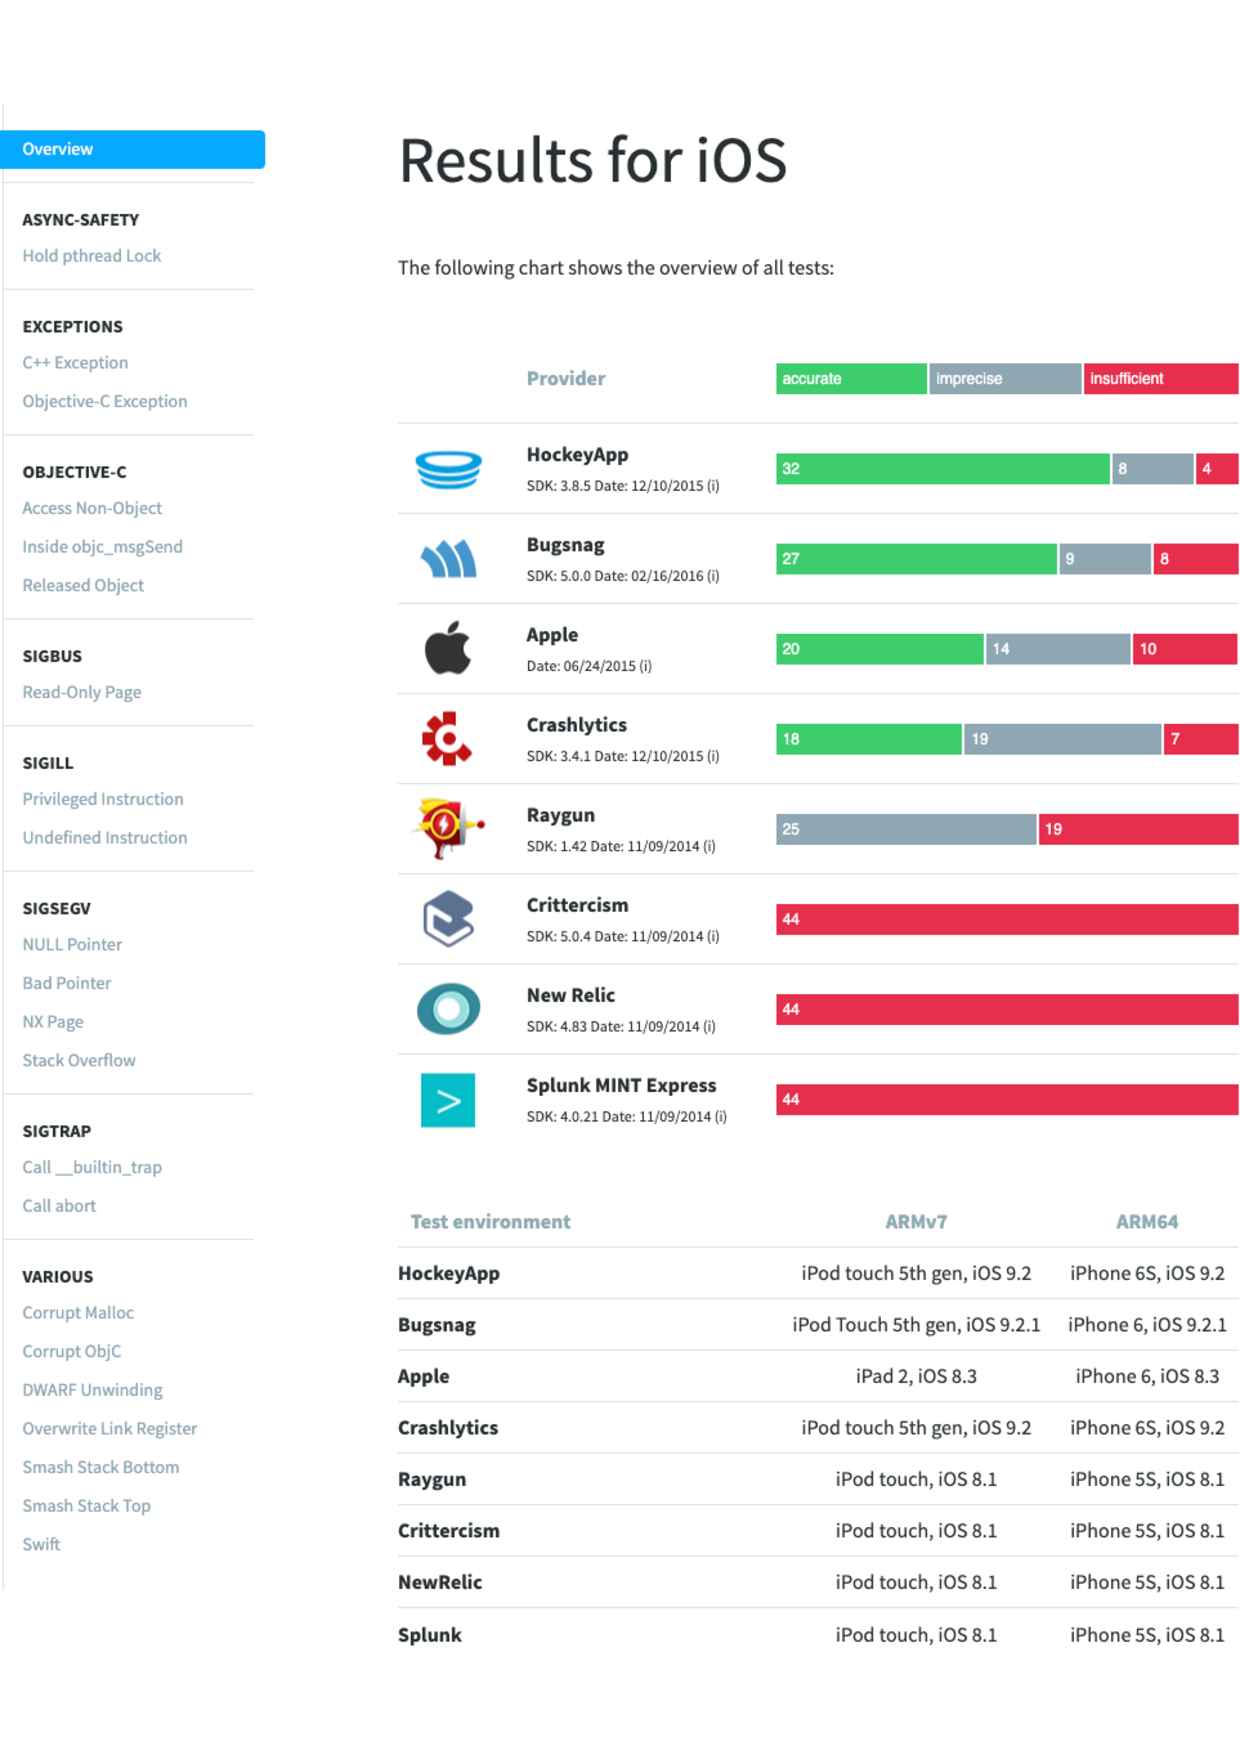
\includegraphics[width=\linewidth]{images/crashprobe.com/CrashProbe-Results-for-iOS-2016-09-06.pdf}
    \caption{Crashprobe iOS SDL results from \nth{06} Sep 2016}
    \label{fig:crashprobe-ios-results}
\end{figure}


The company who developed what became part of Microsoft App Center's crash reporting, Bit Stadium GmbH, %https://www.crunchbase.com/organization/bit-stadium-gmbh 
developed a set of opensource projects called CrashScope which they and various other providers of crash reporting \Glspl{sdk} used to test the behaviours of their respective \Gls{sdk}. An example of their report, from \nth{6} September 2016, is in Figure \ref{fig:crashprobe-ios-results}. The \href{https://github.com/bitstadium/crashprobe.github.com/commit/30844b9794f7cfd48f35d043f255b58f1f70e7e6}{report was last updated on \nth{8} Jun 2017}, however the site remained online for another 3 years, until \href{https://github.com/bitstadium/crashprobe.github.com/commit/4398b88e263d222ed4d55e1dce59d67de11bfaaa}{\nth{20} Aug 2020}, before disappearing. 
%%%% More links
% https://github.com/bitstadium/CrashProbe
% 

\subsection{Improving the analytics performed}~\label{tats-improving-the-analytics-performed}
The analytics on offer in the current tools are basic and the pre-determined groupings are fixed by the tool / service provider. For the enterprise-level paid-for services Google and Microsoft~\sidenote{For example, for Microsoft App Center, see \href{https://docs.microsoft.com/en-us/appcenter/gdpr/analytics-export}{docs.microsoft.com/en-us/appcenter/gdpr/analytics-export}}\index{Microsoft App Center} provide mechanisms for the data to be exported for their in-app analytics (not for \myindex{Android Vitals} or Google Play Console, as far as I can tell). It is not clear to what extent enterprise customers can configure the analytics that's performed, there was no opportunity to evaluate it in the Industrial case study, \myindex{C1}.\sidenote{Perhaps a topic for future research?}

%%%%% Julian continue from here on 29 Aug 2022
\newthought{Future design? }
The introduction of more options may be useful in terms of a) grouping (\emph{e.g.} to define the groupings for `similar' failure clusters) and b) comparisons (\emph{e.g.} compared to what? what are the commonalities and contrasts between when the app's measured as performing well \emph{vs.} performing badly?)

Hopefully simple facilities such as the ability to search through the failures to find any failure clusters that match would be useful. A recent example is searching for instances of an \texttt{IndexOutOfBoundsException} in the \myindex{Kiwix} custom apps\sidenote{\href{https://github.com/kiwix/kiwix-android/issues/2542}{Index Out of Bounds Exception on Custom App \#2542}} where \myindex{Android Vitals} had to be checked page by page for each app to see if the crash was still happening rather than being able to perform a search of the results online.

Aggregation and mining across the matching clusters would also be useful. Tagging/labelling might also help, \emph{ditto} facilities to cross-reference within and across systems (\emph{c.f.} hyperlinking and reference links.

Another aspect would be helping developers recognise common causes and common failures, and the likely effects of addressing these failures in future. (For example, surely Google's got enough data, Machine Learning, Artificial Intelligence, etc. to be able to predict probable improvements for a specific app).


\section[Discussion]{Discussion on mobile analytics tools and their artefacts}~\label{tata-discussion-section}
Mobile Analytics tools need to evolve to remain current and to attract and retain users. Platform tools have a unique advantage compared to in-app tools as the platform tools can collect data across the entire population~\sidenote{Subject to opt-outs, sampling, network connectivity, and other reasons the data wouldn't be sent from the overall population.}. For the Android platform, Google Play Console and Android Vitals are able to provide comparisons with apps of peers, both peers selected by app store classifications~\sidecite{androiddevelopersblog2021_gpc_powers_better_strategic_decisions_etc} and a custom set selected by the developer~\sidecite{play_console_help_compare_your_apps_android_vitals_and_ratings_with_peer_groups}. 

\subsection{ROI and Fidelity}
TODO discuss ROI and Fidelity aspects drawing on various improvements mentioned in \secref{tata-fitness-for-purpose-section} and flaws \secref{tata-flaws-topic}.

\newthought{Return On Investment (ROI): } developers may make both implicit and explicit choices on what to invest in, for instance in terms of their focus, their effort, and their money. The analytics tools need to convince developers a) to invest and then b) whether to increase that investment (and if so what forms of investment e.g. in terms of writing more code, spending [more] money, using the tool more, etc.).
    
\newthought{Fidelity: }
an accurate, faithful representation. In \secref{tata-fidelity-topic} differences of up to 30 fold were reported by developers in the results presented by different mobile analytics. Fidelity does not seem to have been a topic for research in software analytics generally, for instance it's not mentioned (and nor are threats to validity) in the work of Microsoft where they used software analytics within their Lync Windows software (a forerunner to Skype for Business)\sidecite{musson2013_leveraging_the_crowd_how_48000_users_helped_improve_lync_performance}. There seems to be an implicit assumption the reports and measurements are correct, at least in terms of what has been published on the topic. This research has considered fidelity as a topic and also includes some preliminary measurements and results of flaws in the fidelity.


\subsection{Ethical considerations}
The data collected by mobile analytics may have ethical implications a) for the operator/provider of the service, b) for their partners and customers, c) for the developers, d) for end-users. In this research our main focus is on the implications for the developers, nonetheless the other aspects are also important.

As the Catrobat team discovered when they migrated from Fabric to Firebase there were the additional, unexpected analytics that appeared. They considered this sufficiently unethical and intrusive that they removed the product from their mobile app.


\subsection{Some limits of what can be measured}
Together with considerations on fidelity is that of what the client-side \Gls{sdk} is able to measure, because what it doesn't measure is not going to be reported on by the mobile analytics. 

There are areas where the runtime can prevent some pertinent information being collected by some \Glspl{sdk}, for example: \myindex{React Native} runtime - within runtime crashes vs. application crashes where the runtime container crashes, which applied to two of the app-centric case study apps: (\myindex{LocalHalo} and Taskinator\index{GTAF!Taskinator}).

The other is where failures occur to early or too late in the runtime, for example crashes at startup as raised in the email correspondence with Google when comparing Android Vitals with Firebase Crashlytics.

%A placeholder until the relevant content is added to check the formatting in the index for: Android Vitals\index{GitHub Projects!Android Vitals}

\section{Summary of tools and their artefacts}~\label{tata-summary-section}
Despite the various flaws identified in this chapter in the various mobile analytics tools, overall in many cases they helped the various development teams address a subset of the issues. Nonetheless, there is plenty of scope to improve the efficacy of the tools.